\documentclass[10pt,a4paper]{report}


\usepackage{amsmath}
\usepackage[utf8]{inputenc}
\usepackage{amsmath}
\usepackage{amsfonts}
\usepackage{amssymb}
\usepackage{calrsfs}
\usepackage[left=2cm,right=2cm,top=2cm,bottom=2cm]{geometry}
\usepackage[mathscr]{euscript}

%%%for drawing commutative diagrams.%%%%%%
\usepackage{tikz-cd}  
%%%%%%%%%%%%%%%%%%%%%%%%%%%%%%%%%%%%%%%%%%

%%%%%%%%%%for writing large parallel%%%%%%
\usepackage{mathtools}
\DeclarePairedDelimiter\bignorm{\lVert}{\rVert}
%%%%%%%%%%%%%%%%%%%%%%%%%%%%%%%%%%%%%%%%%%

%%%%%%%%%%for changing margin
\def\changemargin#1#2{\list{}{\rightmargin#2\leftmargin#1}\item[]}
\let\endchangemargin=\endlist 

\newenvironment{proof}
{\begin{changemargin}{1cm}{0.5cm} 
	}%your text here
	{\end{changemargin}
}

\newenvironment{subproof}
{\begin{changemargin}{0.5cm}{0.5cm}
	}%your text here
	{\end{changemargin}
}
%%%%%%%%%%%%%%%%%%%%%%%%%%%%%

\begin{document}
\newcommand{\thm}{\textbf{Theorem) }}
\newcommand{\thmnum}[1]{\textbf{Theorem #1) }}
\newcommand{\defi}{\textbf{Definition) }}
\newcommand{\lem}{\textbf{Lemma) }}
\newcommand{\lemnum}[1]{\textbf{Lemma #1) }}
\newcommand{\prop}{\textbf{Proposition) }}
\newcommand{\pf}{\textbf{proof) }}
\newcommand{\cor}{\textbf{Corollary) }}
\newcommand{\cornum}[1]{\textbf{Corollary #1) }}

\newcommand{\lap}{\triangle} %%Laplacian
\newcommand{\s}{\vspace{10pt}}
\newcommand{\bull}{$\bullet$}
\newcommand{\sta}{$\star$}
\newcommand{\reals}{\mathbb{R}}

\newcommand{\eop}{\hfill  \textsl{(End of proof)} $\square$} %end of proof

\newcommand{\intN}{\mathbb{Z}_N}
\newcommand{\norms}[2]{\bignorm[\big]{#1}_{#2}}
\newcommand{\abs}[1]{\big| #1 \big|}
\newcommand{\avg}{\mathbb{E}}
\newcommand{\borel}{\mathscr{B}}
\newcommand{\setlimsup}[2]{\bigcap_{#1=1}^{\infty}\bigcup_{#2=#1}^{\infty}}
\newcommand{\dlim}{D-\lim}
\newcommand{\clim}{C-\lim}

\newcommand{\newday}{======================================================================}
\newcommand{\digression}{**********************************************************************************************}

\setlength\parindent{0pt}
\noindent

\chapter*{Topics in Ergodic Theory}
\s

=====================================================================================
(4th October 2018, Thursday)
\s

\section*{1. Measure preserving system}

\textbf{Measure preserving system} : $(X, \borel, \mu, T)$, where $X$ is a set, $\borel$ is a $\sigma$-algebra, $\mu$ is a probability measure with $\mu(A) \geq 0$ $\forall A \in \borel$, $\mu(X)=1$, and $T$ is a measure-preserving transformation. That is, $T: X\rightarrow X$ is measurable s.t. $\mu(T^{-1}(A)) = \mu(A)$ $\forall A \in \borel$.
\s

If $Y$ is a random element of $X$ with distribution $\mu$, then $T(Y)$ also has distribution $\mu$.
\s

\textbf{Example)}

\begin{itemize}
\item (Circle rotation) Let $X = \reals/ \mathbb{Z}$, $\borel$ be the Borel sets, $\mu$ be the Lebesgue measure and $T = R_{\alpha}$ where $R_{\alpha}(x) = x+\alpha$, and $\alpha \in \reals/\mathbb{Z}$ is parameter.

\item (Times 2 map) $X = \reals/\mathbb{Z}$, $\borel$ be the Borel sets, $\mu$ is a Lebesgue measure, $T = T_2$ where $T_2(x) = 2x$.

\begin{itemize}
\item[ ] \textsl{(proof that $T_2$ is measure preserving)} First prove for intervals : let $I = (a,b)$. Then $\mu(I) = b-a$ and $\mu(T_2^{-1} I)= \mu((\frac{a}{2},\frac{b}{2}) \cup (\frac{a+1}{2},\frac{b+1}{2})) = b/2 - a/2 + b/2 - a/2 = b-a$.(Just use Dynkin's lemma to conclude... Or,)

Now let $U \subset \reals / \mathbb{Z}$ be open. Then $U = \sqcup_{i} I_i$ is a disjoint union of intervals, so
\begin{align*}
\mu(T^{-1}U) = \mu(\sqcup_j T^{-1}I_j) = \sum_j \mu(T^{-1} I_j) = \sum_{j} \mu(I_j) = \mu(U)
\end{align*}

Let $K \subset \reals/\mathbb{Z}$ be a compact set. Then
\begin{equation*}
\mu(T^{-1}K) = 1- \mu((T^{-1}K)^c) = 1- \mu(T^{-1}(K^c)) = 1- \mu(K^c) = \mu(K)
\end{equation*}

Let $A$ be an arbitrary Borel set and let $\epsilon >0$. Then $\exists U$ open and $\exists K$ compact such that $K\subset A \subset A$ and $\mu(U \backslash K) < \epsilon$, so
\begin{align*}
\mu(K) = \mu(T^{-1} K) \leq \mu(T^{-1} A) \leq \mu(T^{-1} U) = \mu(U)
\end{align*}

We also have $\mu(K) \leq \mu(A) \mu(U)$. Since $\mu(U) - \mu(K) < \epsilon$, $|\mu(A) - \mu(T^{-1}A) | < \epsilon$. Since $\epsilon$ was arbitrary, so $\mu(A) = \mu(T^{-1} A)$.

\eop
\end{itemize}
\end{itemize}
\s

The \textbf{orbit} $x \in X$ is the sequence $x, Tx, T^2 x, \cdots$.
\s

Some Questions:

\begin{itemize}
\item Let $A \in \borel$ and $ x\in A$. Doest the orbit of $x$ visit $A$ infinitely often?

\item What is the proportion of the times $n$ such that $T^n x$ is in $A$? 

\item (Mixing property) What is $\mu(\{x \in A : T^nx \in A\})$ if $n$ is large
\end{itemize}
\s

\textbf{Example)} Let $A = [0,\frac{1}{4}) \subset \reals/\mathbb{Z}$ and $T = T_2$. Then $T^n x \in A \Leftrightarrow (n+1)^{\text{st}}$ and $(n+2)^{\text{nd}}$ binary digits of $x$ are 0.

For example, $x = 1/6 = 0.00101010\ldots_{(2)}$ never comes back to $A$.

Another interesting fact : $\mu(\{x : x\in A, T_2^n x \in A \}) = 1/16$ if $n\geq2$.(Circle rotation has very different property.)
\s

\subsection*{Markov Shift}

\begin{itemize}
\item Let $(p_1, p_2, \cdots, p_n)^T$ be a probability vector. Let $A \in \reals_{\geq 0}^{n\times n}$ be the \textbf{matrix of transition probabilities}.

Assumptions : (1) $A(1,\cdots,1)^T = (1,\cdots,1)^T$; (2) $(p_1, \cdots, p_n) A = (p_1, \cdots, p_n)$

\item Let $X = \{ 1,\cdots,n\}^{\mathbb{Z}}$, $\borel$ be the Borel $\sigma$-algebra generated by the product topology of the discrete topology on $\{1,\cdots, n\}$, and $T = \sigma$ is the shift map $(\sigma X)_m = X_{m+1}$.

\item Let $\mu(\{x\in X : x_m=i_0,\cdots,x_{m+n}=i_n\}) = p_{i_0} a_{i_0 i_1} \cdots a_{i_{n-1} i_n}$.
\end{itemize}
\s

\section*{2. Furstenberg's correspondence principle}

\thm (Szemer\'{e}di) Let $S \subset \mathbb{Z}$ of positive upper Banach density. That is:
\begin{align*}
\bar{d}(S) = \limsup_{N,M : M-N \rightarrow \infty} \frac{1}{M-N}|S \cap [N,M-1] | >0.
\end{align*}

Then $S$ contains arbitrary long arithmetic progressions. That is, $\forall l$, $\exists a \in \mathbb{Z}$, $d\in \mathbb{Z}_{>0}$ such that $a, a+d, \cdots, a+(l-1)d \in S$.
\s

\thm (Furstenberg) (Multiple recurrence) Let $(X,\borel,\mu, T)$ be a MPS(Measure preserving system). Let $A \in \borel$ be s.t. $\mu(A) >0$. Let $l\in \mathbb{Z}_{>0}$. Then
\begin{align*}
\liminf_{N\rightarrow \infty} \frac{1}{N} \sum_{n=1}^N \mu(A\cap T^{-n}(A) \cap \cdots \cap T^{-(l-1)n}(A))>0
\end{align*}
\s

=====================================================================================
(6th October 2018, Saturday)
\s

\thm (Szemer\'{e}di) Let $S \subset \mathbb{Z}$ of positive upper Banach density. Then $S$ contains arbitrary long arithmetic progressions. \s

\thm (Furstenberg) Let $(X,\borel,\mu, T)$ be a MPS. Let $A \in \borel$ be s.t. $\mu(A) >0$. Then for $\forall l\in \mathbb{Z}_{>0}$
\begin{align*}
\liminf_{N\rightarrow \infty} \frac{1}{N} \sum_{n=1}^N \mu(A\cap T^{-n}(A) \cap \cdots \cap T^{-(l-1)n}(A))>0
\end{align*}
\s
\s

Let $X =\{0,1\}^{\mathbb{Z}}$, $\borel$ be the Borel $\sigma$-algebra, $T=\sigma$ be the shift map.

For a set $S \subset \mathbb{Z}_{\geq 0}$, Let $x^S \in X$ be defined by
\begin{align*}
x_n^S =\begin{cases}
1 \quad \text{if} \quad n\in S\\
0 \quad \text{if} \quad \text{o/w} 
\end{cases}
\end{align*}

Let $A \in \borel$ and $A = \{x\in X:x_0=1 \}$

Observation : $n\in S \Leftrightarrow \sigma^n x^S \in A \Leftrightarrow (\sigma^n x^S)_0=1 \Leftrightarrow x_n^S =1$.

Let $\{M_m\}$ and $\{N_m\}$ be sequences s.t.
\begin{align*}
\bar{d}(S) = \lim_{m\rightarrow \infty} \frac{1}{M_m - N_m} \big|S \cap [N_m,M_m-1] \big|
\end{align*}
Let $\mu_m = \frac{1}{M_m - N_m} \sum_{n=N_m}^{M_m-1} \delta_{\sigma^n x^S}$, where $\delta_x$ is a measure on $X$ defined as
\begin{align*}
\delta_x(B) = \begin{cases}
1 \quad x\in B \\
0 \quad \text{o/w}
\end{cases}
\end{align*}

Let $\mu$ be the weak limit of a subsequence of $\mu_m$.
\s

\begin{itemize}
\item[ ] \textsl{(Reminder)}

\item \textbf{Weak Limits) : }(In fact, weak-* limits) Let $X$ be a compact metric space, Let $\mu_m$ be a sequence of Borel measures on $X$, and let $\mu$ be another Borel measure. Then $\mu_m$ weakly converges to $\mu$. In notation,
\begin{align*}
\lim-w_{m\rightarrow \infty} \mu_m = \mu
\end{align*}
if $\int f d\mu_m \rightarrow \int f d\mu$ $\forall f\in C(X)$

\item \thm (Banach-Alaoglu/Helly) Let $X$ be a compact metric space. Then $\mathscr{M}(X)$, the set of Borel probability measures endowed with the topology of weak convergence, is compact and metrizable.

In particular, there is a weakly convergent subsequence in any sequence of Borel probability measures.
\end{itemize}
\s

\lem Let $(X,\borel, \mu, \sigma)$ be as defined above is a measure preserving system.
\begin{itemize}
\item[ ] \textbf{proof sketch)} Let $B\in \borel$ Then:
\begin{align*}
\mu_m(B) &= \frac{1}{M_m-N_m} |\{ n \in [N_m, M_m-1] : \sigma^n x^S \in B \}  | \\
\mu_m(\sigma^{-1}B) &= \frac{1}{M_m-N_m} | \{n\in [N_m, M_m -1]:\sigma^n x^S \in \sigma^{-1} B \} | \\
&= \frac{1}{M_m-N_m} | \{n\in [N_m +1, M_m]:\sigma^n x^S \in B \} | \\
|\mu_m(B) - \mu_m(\sigma^{-1}B)| &\leq \frac{1}{M_m-N_m} \rightarrow 0 \quad \text{as } m\rightarrow \infty
\end{align*} 
It can be shown that we can pass to the limit and conclude $\mu (B) = \mu(\sigma^{-1}B)$.
\end{itemize}
\s

\bull \textbf{Remark :} If $B$ is a cylinder set, i.e. $\exists L \in \mathbb{Z}_{>0}$ and $\tilde{B} \subset \{0,1\}^{2L+1}$ s.t.
\begin{align*}
B = \{ x\in X : (x_{-L},\cdots,x_L) \in \tilde{B} \}
\end{align*}
then $B$ is both closed and open. Therefore $\chi_B$, the characteristic function of $B$, is continuous. Hence, the limit
\begin{align*}
\lim_{m\rightarrow \infty} \mu_m(B) = \mu(B)
\end{align*}
\s

\prop Let $S\subset\mathbb{Z}$, let $x^S$, $A$, $(X,\borel, \mu, \sigma)$ be as defined above. Let $l\in \mathbb{Z}_{>0}$. Suppose that $\exists n \in \mathbb{Z}_{>0}$ s.t.
\begin{align*}
\mu ( A \cap \sigma^{-n}(A) \cap \cdots \cap \sigma^{-n(l-1)}(A) ) >0
\end{align*}
Then $S$ contains an arithmetic progression of length $l$.

\begin{proof}
\pf Without loss of generality, we may assume that $\mu = \lim_{m\rightarrow \infty} \mu_m$(if this is not the case, we just replace $\mu_m$ with its converging subsequence).  Let $B = A \cap \sigma^{-n}(A) \cap \cdots \cap \sigma^{-n(l-1)}(A)$ and observe that $B$ is a cylinder set. Then $\mu(B) = \lim \mu_m(B)$ hence $\exists m$ s.t. $\mu_m (B) >0$.

By definition of $\mu_m$, $\exists k \in [N_m,M_m-1]$ such that $\sigma^k x^S \in B$. Hence
\begin{align*}
&\sigma^k x^S \in A, \,\, \sigma^kx^S \in \sigma^{-n}(A),\cdots,\sigma^k x^S \in \sigma^{-n(l-1)}(A) \\
\Rightarrow &\sigma^k x^S \in A, \,\, \sigma^{k+n}x^S \in A, \cdots,\sigma^{k+n(l-1)} x^S \in A
\end{align*}
and so $k,k+n,\cdots,k+n(l-1) \in S$ by earlier observation.

\eop
\end{proof}
\s

Note $A$ is also a cylinder set. Then $\mu(A)= \lim_{m} \mu_m (A)$ and
\begin{align*}
\mu(A) = \lim_m \mu_m(A) = \lim_m \frac{1}{M_m -N_m} \big| \{ n\in [N_m, M_m-1] : n\in S \} \big| = \bar{d}(S) > 0
\end{align*}
by assumption that $S$ is of positive upper Banach density, and therefore we can prove Szemer\'{e}di when assuming Furstenberg.
\s

========================================================================================================
(9th October, Tuesday)
\s

\section*{3. Poincar\'{e} recurrence, Ergodicity}

\lem Let $(X, \borel, \mu, T)$ be MPS. Let $A\in \borel$ with $\mu(A) >0$. Then $\exists n \in \mathbb{Z}_{>0}$ s.t. $\mu(A \cap T^{-n}A) >0$.
\begin{proof}
\pf Suppose $\mu(A \cap T^{-n}A) =0$ for all $n>0$. Then
\begin{align*}
\mu(T^{-k}A\cap T^{-n}A) = \mu(A \cap T^{-(n-l)}A ) =0
\end{align*}
for all $n>k\geq 0$. Hence the sets $A, T^{-1}A,\cdots$ are "almost pairwise disjoint". Then
\begin{align*}
\mu(A \cup T^{-1}A \cup \cdots \cup T^{-n}A) &= \mu(A) + \big( \mu(T^{-1}A) - \mu(T^{-1}A \cap A) \big)\\
& + \big( \mu(T^{-2}A) - \mu(T^{-2}A \cap (A \cup T^{-1}A)) + \cdots \\
& + \big( \mu(T^{-n}A) - \mu(T^{-n}A \cap (A \cup T^{-1}A \cup \cdots \cup T^{-(n-1)}A) ) \big) \\
& = (n+1) \mu(A),
\end{align*}
a contradiction if $n+1 > \mu(A)^{-1}$.

\eop
\end{proof}
\s

\thm (Poincar\'{e} recurrence) Let $(X,\borel, \mu, T)$ be MPS. Let $A \in \borel$ with $\mu(A) >0$. Then a.e. $x\in A$ returns to $A$ infinitely often. That is,
\begin{align*}
\mu(A \backslash \setlimsup{N}{n} T^{-n} A  ) =0
\end{align*}
\s

\textbf{Remark : } $x\in T^{-n} A$ $\Leftrightarrow$ $T^{n}x \in A$. So $\cup_{n=N}^{\infty} T^{-n}A$ are the points that visit $A$ at least once after time $N$. 
\s

\begin{proof}
\pf Let $A_0$ be the set of point in $A$ that never returns to $A$. We first show $\mu(A_0)=0$. Note that $\mu(A_0 \cap T^{-n}A_0) \leq \mu(A_0 \cap T^{-n}A) = \mu(\phi) =0$ for all $n>0$. By the previous lemma, we have $\mu(A_0) =0$. Note that if $x\in A \backslash \big( \setlimsup{N}{n} T^{-n} A \big)$, then there is a maximal $m\in \mathbb{Z}_{\geq 0}$ such that $T^{m}x \in A_0$. This means that
\begin{align*}
A \backslash \cap \cup T^{-n} A \subset \cup_{m=0}^{\infty}T^{-m}A_0
\end{align*}
and since $T^{-m} A_0$ has measure 0 for each $m\geq 0$, $A \backslash \cap \cup T^{-n} A$ also has measure 0.

\eop
\end{proof}
\s

However, if we are aim to show that any point of $X$(or almost every) visits a set $A$ with $\mu(A)$ infinitely often, we should prevent elements of $X$ being partitioned by orbits of $T^{-1}$. Assumption of ergodicity turns out to be enough for this.(In fact, we can make 'ergodic decomposition' for $T$ to to satisfy ergodicity on each partition - but not lecturing on this; bit tricky)
\s

\defi A MPS $(X,\borel, \mu, T)$ is called \textbf{ergodic} if $A=T^{-1}A$ implies $\mu(A) =0$ or $1$ for all $A \in \borel$.
\s

If the MPS is not ergodic, and $A \in \borel$ with $\mu(A) \in (0,1)$ s.t. $T^{-1}A =A$, then we can restrict the MPS to $A$. That is, we consider the MPS:

\quad $(A,\borel_A, \mu_A, T\big|_A)$ where $\borel_A = \{B\in \borel : B \subset A \}$, $\mu_A(B) = \mu(B)/\mu(A)$ for all $B\in \borel_A$.
\s

\thm The following are equivalent for a MPS $(X,\borel, \mu, T)$ :
\begin{itemize}
\item[(1)] $(X,\borel, \mu, T)$ is ergodic.
\item[(2)] $\mu(\setlimsup{N}{n} T^{-n} A ) =1$ for all $A\in \borel$ with $\mu(A) >0$.
\item[(3)] $\mu(A \bigtriangleup T^{-1} A) =0$ implies $\mu(A) =0$ or 1 for all $A\in \borel$.
\item[(4)] For all bounded measurable functions $f:X\rightarrow \reals$, $f = f \circ T$ a.e. implies $f$ is constant a.e.
\item[(5)] For all measurable functions $f:X\rightarrow \mathbb{C}$, $f = f \circ T$ a.e. implies $f$ is constant a.e.
\end{itemize}
\s

Each condition show different perspective to view ergodicity. The second item shows that for ergodic systems Poincar\'{e} recurrence holds in a stronger form: not only almost every point in $A$ but also almost every point in $X$ visits $A$ infinitely often. The last three conditions are often used in practice.
\begin{proof}
\pf \begin{itemize}
\item[(1)$\Rightarrow$(2)] Let $A\in \borel$ with $\mu(A) >0$ Let $B = \bigcap \bigcup T^{-n}A$, the set of points that visit $A$ infinitely often. By Poicar\'{e} recurrence(or P-recurrence), $\mu(B) \geq \mu(A) >0$. So if we show that $B = T^{-1}B$, then $\mu(B)=1$ follows by ergodicity.

\quad While, $x\in B$ $\Leftrightarrow$ $x$ visits $A$ i.o. $\Leftrightarrow$ $Tx$ visits A i.o. $\Leftrightarrow$ $Tx \in B$. So we proved $B = T^{-1}B$.
\item[(2)$\Rightarrow$(3)] Let $A\in \borel$ s.t. $\mu(A \bigtriangleup T^{-1} A) =0$. If $\mu(A) =0$, there is nothing to prove, so assume $\mu(A)>0$. Let $B= \cap \cup T^{-n} A$. By (2), we know that $\mu(B) = 1$. We show $\mu(B\backslash A) =0$, which completes the proof.

\quad Let $x\in B\backslash A$, then there is a first time $m>0$ s.t. $T^m x\in A$, hence $x\in T^{-m}A \backslash T^{-(m-1)}A$. This shows $B\backslash A \subset \bigcup T^{-m} A \backslash T^{-(m-1)A}$. But $T^{-m} A \backslash T^{-(m-1)A}$ has measure 0 because $\mu(T^{-m} A \backslash T^{-(m-1)}A)= \mu(T^{-1}A\backslash A) =0$.

\quad So we conclude $\mu(B\backslash A) =0$.
\item[(3)$\Rightarrow$(4)] Let $f:X\rightarrow \reals$ be a bounded measurable function s.t. $f= f\circ T$ almost everywhere. For any $t\in \reals$, define $A_t = \{x\in A : f(x) \leq t\}$. Then
\begin{align*}
\mu(A_t \bigtriangleup T^{-1}A_t) = \mu( \{x\in A : f(x) \leq t\} \bigtriangleup \{x\in A : f \circ T(x) \leq t\}) =0
\end{align*} 
By (3), we have $\mu(A_t)\in \{0,1\}$ for all $t$. Since $f$ was bounded, if $t$ is very small, then $\mu(A_t)=0$ and if $t$ is very large $\mu(A_t) =1$. But $t\mapsto \mu(A_t)$ is a monotone function, we have $\exists c \in \reals$ s.t. $\mu(A_t) =0$ for all $t<c$ and $\mu(A_t) =1$ for all $t>c$. Therefore we have $f(x)=c$.
\item[(4)$\Rightarrow$(1)] Let $A\in \borel$ with $A = T^{-1}A$. Then $\chi_A = \chi_A \circ T$ everywhere, so $\chi_A$ is constant a.e.
\end{itemize}
\end{proof}
\s

\textbf{Example :} The circle rotation $(\reals/\mathbb{Z},\borel, \mu, R_{\alpha})$ is ergodic if and only if $\alpha$ is irrational.

\begin{proof}
\pf Let $f:X\rightarrow \reals$ be measurable, and let $f(x) = \sum_{n\in \mathbb{Z}} a_n \exp(2\pi i nx)$. Then
\begin{align*}
f\circ R_{\alpha}(x) = f(x+\alpha) &= \sum_{n\in \mathbb{Z}}a_n \exp(2\pi in (x+\alpha)) \\
&= \sum_{n\in \mathbb{Z}} a_n \exp(2\pi in\alpha) \exp(2\pi i nx)
\end{align*}
so $f=f\circ R_{\alpha}$ is equivalent to having $a_n = a_n \exp(2\pi i n \alpha)$ for all $n$.
If $\alpha$ is irrational, then $\exp(2\pi in\alpha) \neq 1$ for all $n\neq 0$ so $a_n=0$ for all $n\neq 0$.

\eop
\end{proof}
\s

\newday

(11th October, Thursday)
\s

\section*{4. Ergodic theorems}

\thm (Mean ergodic theorem, von Neumann) Let $(x,\borel, \mu, T)$ be a MPS. Write
\begin{align*}
I = \{ f\in L^2(X) : f\circ T = f \,\,\, \text{a.e.} \}  \subset L^2(X)
\end{align*}
for the closed subspace of $T$-invariant functions. Write $P_T : L^2(X) \rightarrow I$ for the orthogonal projection. Then for every $f\in L^2(X)$, we have
\begin{align*}
\frac{1}{N} \sum_{n=0}^{N-1} f\circ T^n \rightarrow P_T f \quad \text{in } L^2(X)
\end{align*}
Here, $\frac{1}{N} \sum_{n=0}^{N-1} f\circ T^n$ called the \textbf{ergodic average}.
\s

There are two proofs for this theorem : one uses spectral theory and the the other does not. We would prove using the second approach, and sketch the first proof in the example sheet.

\s

\thm (Pointwise ergodic theorem, Birkhoff) Let $(X,\borel, \mu, T)$ be a MPS. Then for all $f\in L^1(X)$, $\exists f^* \in L^1(X)$ s.t. $f^* = f^* \circ T$ a.e. and 
\begin{align*}
\frac{1}{N} \sum_{n=0}^{N-1} f\circ T^n (x) \rightarrow f^*(x) \quad \text{a.e. in } X 
\end{align*}
\s

\textbf{Comments}
\begin{itemize}
\item[(1)] If $f\in L^2 \cap L^1$, then $f^* = P_T f$.
\item[(2)] There is an $L^p$ version of convergence in norm. That is, if $f\in L^p$, then
\begin{align*}
\frac{1}{N} \sum_{n=0}^{N-1} f\circ T^n \rightarrow f^* \quad \text{in } L^p \text{ norm}
\end{align*}
This will be proved in the example sheet.
\item[(3)] If $(X,\borel, \mu, T)$ is ergodic, then $f^*$(or $P_T f$) is constant a.e., because it is $T$-invariant.

\quad Note : $f^*(x)  = \int f^* d\mu$ a.e. By $L^1$ norm convergence, we also have
\begin{align*}
\lim_{N\rightarrow \infty} \int \frac{1}{N} \sum_{n=0}^{N-1} f\circ T^n d\mu \rightarrow \int f^* d\mu
\end{align*}
By a lemma that would follow,
\begin{align*}
\int f\circ T^n d\mu = \int fd\mu \quad \forall n, \text{ hence} \quad \int f d\mu = \int f^* d\mu
\end{align*}
Then
\begin{align*}
\frac{1}{N} \sum_{n=0}^{N-1}f(T^n x) \rightarrow \int f d\mu
\end{align*}
Can be interpreted as "time average(LHS) converges to spatial average(RHS)".
\end{itemize}
\s

\lem Let $T : X \rightarrow X$ be a measurable transformation and let $\mu$ be a probability measure. Then $\mu$ is $T$-invariant \emph{if and only if}
\begin{align}
\int f\circ T d \mu = \int f d\mu \quad \forall f \in L^1(X,\mu)  \label{*}
\end{align}
\begin{proof}
\pf  (\emph{(\ref{*}) $\Rightarrow$ measure preserving property}) : Let $A\in \borel$. Then
\begin{align*}
\mu(T^{-1} A) = \int \chi_{T^{-1} A} d\mu = \int \chi_A \circ T d\mu = \int \chi_A d\mu = \mu(A)
\end{align*}

(\emph{MPP $\Rightarrow$ (\ref{*})}) : Let $f\in L^1(X)$. If $f= \chi_A$ for some $A\in \borel$, then
\begin{align*}
\int f \circ T d\mu = \mu(T^{-1}A) = \mu (A)  = \int f d\mu
\end{align*}
(\ref{*}) hold for such $f$. Then (\ref{*}) also holds for simple functions by linearity of integration. In the case where $f$ is non-negative, let $f_n$ be a monotone increasing sequence of simple functions such that $\lim_n f_n = f$(e.g. $f_n = f\wedge n$),
\begin{align*}
\int f\circ T d\mu = \lim_n \int f_n \circ T d\mu = \lim_n \int f_n d\mu = \int fd\mu
\end{align*}
\quad In the general case, separate $f$ into positive and negative parts and conclude the proof.

\eop
\end{proof}
\s

\defi Let $(X,\borel, \mu, T)$ be a MPS. Then the \textbf{Koopman operator} is defined as : $U_T f = f\circ T$ acting on functions on $X$.
\s

\lem The Koopman operator is an isometry on $L^2(X)$. That is,
\begin{align*}
\langle f,g\rangle = \langle U_T f, U_T g \rangle
\end{align*}
\begin{proof}
\pf Apply the previous lemma for the function $f\circ \bar{g}$.
\begin{align*}
\mu(U_T f \cdot U_T \bar{g}) = \mu(U_T(f\bar{g})) = \mu(f\bar{g})
\end{align*}

\eop
\end{proof}
\s

\defi A MPS $(X,\borel, \mu, T)$ is called \textbf{invertible} if $\exists S:X\rightarrow X$, measure preserving, s.t.
\begin{align*}
S\circ T = T\circ S= id_X \quad \text{a.e.}
\end{align*}
If such a map exists, we denote it by $T^{-1} = S$. (such operator is unique up to a.s. equality)
\s

\lem If $(X,\borel, \mu, T)$ is invertible, then $U_T$ is unitary, and $U^*_T = U_{T^{-1}}$.

\begin{proof}
\pf Note : $U_{T^{-1}} \circ U_T = U_T \circ U_{T^{-1}} = id_{L^2(X)}$, so it is enough to show that $U^*_T = U_{T^{-1}}$. To do this, we need to show :
\begin{align*}
\langle U_{T^{-1}} f, g\rangle = \langle f, U_T g\rangle \quad \forall f,g, \in L^2
\end{align*}
and
\begin{align*}
\langle U_{T^{-1}} f, g\rangle = \int f\circ T^{-1} \cdot \bar{g} d\mu = \int \Big( f\circ T^{-1} \cdot \bar{g}  \Big) \circ T d\mu = \int f\cdot \bar{g} \circ T d\mu = \langle f, U_T g\rangle
\end{align*}

\eop
\end{proof}
\s

\quad Both von Neumann's and Birkhoff's theorems are easy for certain special kinds of functions. For instance, if $f\in I$ :
\begin{align*}
\frac{1}{N} \sum_{n=0}^{N-1} f\circ T^n =f
\end{align*}
Also, if $f= g \circ T -g$ for some $g$, then
\begin{align*}
\frac{1}{N} \sum_{n=0}^{N-1} f\circ T^n = \frac{1}{N}\big( g\circ T^N - g \big)
\end{align*}
It turns out that these two are the only functions that we have to worry about (in the case of von Neumann's theorem) - as presented in the following lemma.
\s

\lem Write $B = \{g\circ T-g:g\in L^2(x) \}$. Then $B^{\perp} =I$.
\s

\textit{Caution ! :} $B$ is not close in $L^2$. So we get $L^2 = I \oplus \bar{B}$, but not $L^2 = I \oplus B$. 

\begin{proof}
\pf Let $f\in L^2(X)$. Then
\begin{align*}
& f\in B^{\perp} \quad \Leftrightarrow \quad \langle f, g\circ T - g\rangle = 0 \quad \forall g \in L^2 \\
\Leftrightarrow \quad & \langle f, g\circ T \rangle = \langle f, g\rangle \quad \forall g \in L^2 \\
\Leftrightarrow \quad & \langle U^*_T f, g\rangle = \langle f, g\rangle \quad \forall g \in L^2 \\
\Leftrightarrow \quad & U^*_T f = f
\end{align*}
Now we only need to see that $U^*_T f=f$ $\Leftrightarrow$ $U_T f =f$ :
\begin{align*}
& U_T f = f \\
\Leftrightarrow \quad &\norms{f-U_T f}{}^2 = 0 \\
\Leftrightarrow \quad & \norms{f}{}^2 + \norms{U_T f}{}^2 - \langle f, U_T f\rangle - \langle U_T f,f\rangle =0 \\
\Leftrightarrow \quad & \norms{f}{}^2 + \norms{U^{*}_T f}{}^2 - \langle f, U^{*}_T f\rangle - \langle U^{*}_T f, f\rangle + \Big( \norms{U_T f} - \norms{U^*_T f}{}^2 \Big) =0 \\
\Leftrightarrow \quad & \norms{f-U^{*}_T f}{}^2 + \Big( \norms{U_T f}{}^2 - \norms{U^{*}_T f}{}^2 \Big) = 0
\end{align*}
Since $\norms{f-U^*_T f}{}^2 \geq 0$, $\norms{U_T f}{}^2 - \norms{U^*_T f}{}^2 \geq 0$(note that we do not know that $U^*_T$ is unitary, since we do not know if $T$ is invertible, but we know that $\norms{U^*_T}{op} \leq 1$), this statement is equivalent to having $f = U^*_T f$.
\end{proof}
\s

Now we are ready to prove the mean ergodic theorem.

\begin{proof}
\textbf{proof of MET) } Fix $\epsilon>0$. Let $f\in L^2$. By the lemma, $\exists g,e \in L^2$ s.t.
\begin{align*}
f= P_T f + (g\circ T -g) +e
\end{align*}
with $\norms{e}{} <\epsilon$ and
\begin{align*}
\frac{1}{N}\sum_{n=0}^{N-1}f\circ T^n = P_T f + \frac{1}{N}(g\circ T^N -g) + \frac{1}{N} \sum_{n=0}^{N-1} e\circ T^n
\end{align*}
This gives bound
\begin{align*}
\norms{\frac{1}{N}\sum_{n=0}^{N-1}f\circ T^n - P_T f}{} \leq \frac{2\norms{g}{}}{N} + \epsilon
\end{align*}
Taking $N\rightarrow \infty$ gives
\begin{align*}
\limsup_{N\rightarrow \infty} \norms{\frac{1}{N} \sum_{n=0}^{N-1} f\circ T^n - P_T f}\leq \epsilon
\end{align*}

\eop
\end{proof}
\s

\newday

(13th October, Saturday)
\s

Now we start proving mean ergodic theorem, starting with the following theorem.
\s

\thm \emph{(Maximal Ergodic Theorem, Wiener)} Let $(X,\borel, \mu, T)$ be a MPS. Let $f\in L^1$, $\alpha\in \reals_{>0}$. Let
\begin{align*}
E_{\alpha} = \{x\in X : \sup_N \frac{1}{N} \sum_{n=0}^{N-1} f(T^n x) > \alpha \}
\end{align*}
Then $\mu(E_{\alpha}) \leq \frac{1}{\alpha} \norms{f}{1}$.
\s

-the theorem is useful, because we can bound some set of particular irregularity depending on the parameter $\alpha$.

-usually, these kinds of maximal inequalities are prove using covering lemmas, e.g. using Vitalli covering lemma. This is also possible in this case, but the proof gets too long.
\s

The proof of the theorem depends on the following proposition
\s

\prop Let $(X,\borel, \mu, T)$ be a MPS. Let $f\in L^1$. Let
\begin{align*}
&f_0 =0, \quad f_1=f, \quad f_2=f\circ T + f, \quad \cdots \\
&f_n = f\circ T^{n-1} + \cdots + f\circ T + f = f_{n-1}\circ T + f \\
&F_N = \max_{n=0,\cdots,N} f_n
\end{align*}
Then $\int_{x:F_N(x)>0} f(x)d\mu(x) \geq 0$ for all $N$.
\begin{proof}
\pf  Suppose that $F_N(x)>0$. Then $F_N(x) =f_n(x)$ for some $n \in \{1,\cdots N\}$. Then $F_N(x) = f_{n-1}(Tx) + f(x) \leq F_N(Tx) +f(x)$, hence $f(x) \leq F_N(x) -F_N(Tx)$.
\begin{align*}
\int_{\{x: F_N(x)>0\}} f(x) d\mu \geq \int_{\{x:F_N(x)>0\}} (F_N(x)-F_N\circ T(x) ) d\mu(x)
\end{align*}
Note, if $F_N(x)\leq 0$, then we have $F_N(x) = 0$ and $F_N(x) - F_N(Tx) \leq 0$, so we have $F_N(x) - F_N \circ T(x) \geq 0$ on the domain $\{x: F_N(x) >0 \}$. 

\eop
\end{proof}
\s

We now prove maximal ergodic theorem.

\begin{proof}
\textbf{proof of Maximal E.T.)} Define
\begin{align*}
E_{\alpha,N} &= \{x\in X : \max_{m=0\cdots, N} \frac{1}{m} \sum_{n=0}^{m-1} f(T^n x) >\alpha   \} \\
&= \{x\in X: \max_{m=0,\cdots,N} \sum_{n=0}^{m-1} \big( f(T^n x) - \alpha \big) > 0 \}
\end{align*}
(with convention that the sum is just 0 in the case $m=0$) We apply the proposition for the function $f-\alpha$. Then
\begin{align*}
\int_{E_{\alpha, N}} \big( f(x) - \alpha \big) d\mu \geq 0
\end{align*}
Then
\begin{align*}
\norms{f}{1} \geq  \int_{E_{\alpha, N}} f(x) \geq \alpha \mu(E_{\alpha,N}) 
\end{align*}
Note that $E_{\alpha} = \bigcup_{M} E_{\alpha,M}$ is an increasing union and the inequality holds for any $N$, so $\norms{f}{1} \geq \alpha\mu(E_{\alpha})$.

\eop
\end{proof}
\s

Note that, in fact the proof in showing a somewhat stronger version of maximal ergodic theorem. Namely,
\s

\thm \emph{(Maximal Ergodic Theorem, version 2)} Let $(X,\borel, \mu, T)$ be a MPS. Let $f\in L^1$, $\alpha\in \reals_{>0}$. Let
\begin{align*}
E_{\alpha} = \{x\in X : \sup_N \frac{1}{N} \sum_{n=0}^{N-1} f(T^n x) > \alpha \}
\end{align*}
Then $\mu(E_{\alpha}) \leq \frac{1}{\alpha} \mu(f 1_{E_{\alpha}} )$.
\begin{proof}
\pf It follows from the fact $\int_{E_{\alpha, N}} f(x) \geq \alpha \mu(E_{\alpha,N}) $ for all $N\geq 0$.

\eop
\end{proof}
\s

\thm (Pointwise ergodic theorem) Let $(X,\borel, \mu, T)$ be a MPS. Let $f\in L^1$. Then $\exists f^* \in L^1$, $T$-invariant s.t.
\begin{align*}
\frac{1}{N} \sum_{n=0}^{N-1} f(T^n x) \rightarrow f^* (x) \quad \text{pointwise a.e.}
\end{align*}
\begin{proof}
\pf Fix $\epsilon >0$. Then $\exists f_{\epsilon} \in L^2$, $e_{\epsilon, 1} \in L^1$ s.t.
\begin{align*}
f = f_{\epsilon} + e_{\epsilon,1}\quad \text{and } \norms{e_{\epsilon,1}}{1} <\epsilon.
\end{align*}
Also $\exists g_{\epsilon} \in L^2$, $e_{\epsilon,2} \in L^2$ s.t.
\begin{align*}
f_{\epsilon} = P_T f_{\epsilon} + g_{\epsilon} \circ T - g_{\epsilon} + e_{\epsilon,2} \quad \text{and } \norms{e_{\epsilon,2}}{1} <\epsilon
\end{align*}
and $\exists h_{\epsilon} \in L^{\infty}$, $e_{\epsilon,3} \in L^1$ s.t.
\begin{align*}
g_{\epsilon} = h_{\epsilon} + e_{\epsilon,3}\quad \text{and } \norms{e_{\epsilon,3}}{1}<\epsilon
\end{align*}

\quad So $f = P_T f_{\epsilon} + h_{\epsilon}\circ T - h_{\epsilon} + e_{\epsilon}$, where $e_{\epsilon} \in L^1$ with$ \norms{e_{\epsilon}}{1} <\epsilon$.
\begin{align*}
\frac{1}{N} \sum_{n=0}^{N-1} f(T^n x) = P_T f_{\epsilon}(x) + \frac{1}{N} \big( h_{\epsilon}(T^n x) - h_{\epsilon}(x) \big) + \frac{1}{N}\sum_{n=0}^{N_1} e_{\epsilon}(T^n x)
\end{align*}
Let
\begin{align*}
E_{\epsilon,\alpha} = \{ x\in : \limsup_{N\rightarrow \infty} \Big| \frac{1}{N} \sum_{n=0}^{N-1} f(T^n x) - P_T f_{\epsilon}(x) > \alpha  \Big| \}
\end{align*} 
(Not same as $E_{\alpha, N}$ defined earlier)
Applying the Maximal ergodic theorem for the $f_n$ gives
\begin{align*}
\mu(E_{\epsilon,\alpha} ) \leq \frac{1}{\alpha} \norms{e_{\epsilon}}{1} \leq \frac{h\epsilon}{\alpha}
\end{align*}

\quad Let $F$ be the set of points $x$ s.t. $\frac{1}{N} \sum_{n=0}^{N_1} f(T^n x)$ does not converge at $x$. Then $F\subset \bigcup_{\alpha}F_{\alpha}$, where
\begin{align*}
F_{\alpha} = \{x\in X : \limsup_{N_1,N_2 \rightarrow \infty} \Big| \frac{1}{N} \sum_{n=0}^{N_1 -1} f(T^n x) - \frac{1}{N_2} \sum_{n=0}^{N_2 -1} f(T^n x) \Big| >2\alpha  \}
\end{align*}
Notice, $F_{\alpha} \subset E_{\epsilon, \alpha}$ for all $\epsilon>0$(?????), so $\mu(F_{\alpha}) \leq \mu(E_{\epsilon,\alpha}) \leq \frac{h \epsilon}{\alpha}$. Therefore $\mu(F_{\alpha}) =0$. We can take a countable sequence of $\alpha$'s(e.g. $(1/k)_{k\in \mathbb{N}}$) and conclude $\mu(F) = 0$.

\quad We proved that $\frac{1}{N} \sum_{n=0} f(T^n x) \rightarrow f^*(x)$ for some function $f^*$. By Fatou's lemma, we have $f^* \in L^1$, and it remains to prove $f^*(x) = f^*(Tx)$ a.e.

\quad For almost every $x$,
\begin{align*}
f^*(x) &= \lim_{N\rightarrow \infty} \frac{1}{N} \sum_{n=0}^{N-1}f(T^n x) \\
f^*(Tx) &= \lim_{N\rightarrow \infty} \frac{1}{N} \sum_{n=0}^{N-1} f(T^{n-1} x) \\
&= \lim_{N\rightarrow \infty} \frac{1}{N} \sum_{n=0}^{N-1} f(T^n x) \\
&= \lim_{N\rightarrow \infty} \frac{1}{N-1} \sum_{n=1}^{N-1} f(T^n x) \\
&= \lim_{N\rightarrow \infty} \frac{1}{N} \sum_{n=1}^{N-1} f(T^n x)
\end{align*}
Therefore $f^*(x) - f^*(Tx) = \lim_{N\rightarrow \infty} \frac{1}{N}f(x) = 0$ 

\eop
\end{proof}

==============================================================================

\begin{proof}
\textbf{a more elegant proof) }
For simplicity, let $S_N(x) \frac{1}{N} \sum_{n=0}^{N-1} f\circ T^n (x)$.
\begin{itemize}
\item[(1)] First, let $f$ be a positive $L^1$ function. Then we may find a positive measurable function $\bar{f}(x)$  such that
\begin{align*}
&\bar{f}(x) = \liminf_{N\rightarrow \infty} S_N(x) \quad \text{a.e.}
\end{align*}
Note that $\bar{f}$ is $T$-invariant, since
\begin{align*}
S_N \circ T = \frac{1}{N}(f\circ T + \cdots + f\circ T^N) = \frac{N+1}{N} S_{N+1} - \frac{1}{N} f
\end{align*} 
Also, by Fatou's lemma,
\begin{align*}
\mu (| \bar{f} |) \leq \liminf_{N} \mu(| \frac{1}{N} \sum_{n=0}^{N-1} f\circ T^n |) = \norms{f}{1} <\infty  
\end{align*}
and therefore $\bar{f} \in L^1$ with $\int \bar{f} d\mu = \int fd\mu$. Now let $g(x) = f(x) - \bar{f}(x)$, then again $g\in L^1$, with $\int g d\mu = 0$ and 
\begin{align*}
\liminf_{N\rightarrow \infty} \frac{1}{N} \sum_{n=0}^{N-1} g\circ T^n (x) =0 \quad \text{a.e.}
\end{align*}
Now consider the set $F_q$, defined for $q\in \mathbb{Q}_{>0}$.
\begin{align*}
F_q = \{  x: \limsup_N  \frac{1}{N} \sum_{n=0}^{N-1} g \circ T^n (x) > q   \}
\end{align*}
Observe that $F_q$ is a $T$-invariant set, since
\begin{align*}
Tx \in F_q \quad &\Leftrightarrow \quad \limsup_{N} \frac{1}{N} \sum_{n=0}^{N-1} g\circ T^{n+1}(x) > q \\
&\Leftrightarrow \quad \limsup_{N} \Big( \frac{1}{N} \sum_{n=0}^{N} g\circ T^{n}(x) -\frac{1}{N} g \Big) > q \quad \Leftrightarrow \quad x\in F_q
\end{align*}
So we may repeat our arguments above to the restricted MPS $(F_q, \borel \big|_{F_q}, \mu\big|_{F_q}, T\big|_{F_q})$ and hence show that $\mu(g 1_{F_q}) = \mu(f 1_{F_q}) - \mu(\bar{f} 1_{F_q}) =0$. But by the maximal ergodic theorem(version 2), we have
\begin{align*}
& q \mu(F_q) \leq  \int_{F_q} g d\mu =0
\end{align*}
hence $\mu(F_q) =0$, and 
\begin{align*}
\mu(\{ x : |\limsup_N  \frac{1}{N} \sum_{n=0}^{N-1} g \circ T^n (x) |>0  \}) = \mu (\cap_{q\in \mathbb{Q}_{>0}} F_q) = 0
\end{align*}
We may conclude that
\begin{align*}
\limsup_N  \frac{1}{N} \sum_{n=0}^{N-1} g \circ T^n (x) = \liminf_N  \frac{1}{N} \sum_{n=0}^{N-1} g \circ T^n (x)  = 0 \quad \text{a.e.}
\end{align*}
and we see that
\begin{align*}
\lim_{N\rightarrow \infty }\frac{1}{N} \sum_{n=0}^{N-1} f \circ T^n (x) \rightarrow \bar{f} \quad \text{a.e.}
\end{align*}
with $\norms{\bar{f}}{1} \leq \norms{f}{1}$.

\item[(2)] For the general case, just divide $f$ into a non-negative part and a negative part, e.g. $f=f^+ - f^-$ and apply part (1) to show that
\begin{align*}
& \lim_{N\rightarrow \infty }\frac{1}{N} \sum_{n=0}^{N-1} f^+ \circ T^n (x) \rightarrow \bar{f}^+ \quad \text{a.e.} \\
& \lim_{N\rightarrow \infty }\frac{1}{N} \sum_{n=0}^{N-1} f^- \circ T^n (x) \rightarrow \bar{f}^- \quad \text{a.e.}
\end{align*}
and put $f^* = \bar{f}^+ - \bar{f}^-$, then we have the desired result.
\end{itemize} 

\eop
\end{proof}
\s

=======================================================================

(not done in the lecture. a question in example sheet.)

\thm (Pointwise ergodic theorem, $L^p$-version) Let $(X,\borel, \mu, T)$ be a MPS, that is $\sigma$-finite. Let $f\in L^p$. Then $\exists f^* \in L^p$, $T$-invariant s.t.
\begin{align*}
\frac{1}{N} \sum_{n=0}^{N-1} f(T^n x) \rightarrow f^* (x) \quad \text{pointwise a.e.}
\end{align*}
\begin{proof}
\pf First, assume that $f$ is a positive function. Let $(f_n)_n$ be a increasing sequence of $L^1$ functions s.t. $f_n \rightarrow f$ in $L^p$ and almost everywhere. Then by pointwise ergodic theorem for $L^1$ functions, we may find $(f^*_n)_n \subset L^1$ s.t.
\begin{align*}
\lim_{N\rightarrow \infty }\frac{1}{N} \sum_{n=0}^{N-1} f_n \circ T^n (x) \rightarrow f^*_n \quad \text{a.e.}
\end{align*}
Then $(f^*_n)_n$ also forms an increasing sequence, and therefore converges almost everywhere, say $f^*_n \rightarrow f^*$ a.e. Now, by Fatou's lemma, we have, for $n\geq m$,
\begin{align*}
\mu( (f^*_n - f^*_m)^{p} )^{1/p} \leq \liminf_{n} \Big( \mu( \frac{1}{N} \sum_{k=0}^{N-1} (f_n - f_m)  \circ T^k )  \Big)^{1/p} \leq \liminf_n \mu((f_n-f_m)^p)^{1/p}
\end{align*}
where the last inequality follows from Minkowski's inequality. Therefore, $(f^*_n)_n$ forms a Cauchy sequence in $L^p$, and in fact converges to $f^*$ in $L^p$. Also, again by Minkowski's inequality, we have $\norms{f^*_n}{p} \leq \norms{f_n}{p}$ and 
\begin{align*}
\norms{\frac{1}{N} \sum_{m=0}^{N-1} f_n \circ T^m}{p} \leq \norms{f_n}{p}
\end{align*}
so by dominated convergence theorem, we realize that $\frac{1}{N} \sum_{n=0}^{N-1} f_n \rightarrow f^*$ is in fact in $L^p$. Putting these results together, we conclude that
\begin{align*}
\frac{1}{N} \sum_{n=0}^{N-1} f \circ T^n \rightarrow f^* \quad \text{in } L^p \text{ and a.e.}
\end{align*}


\begin{center}
\begin{large}
\begin{tikzcd}
f_n \arrow[r, "L^p"] \arrow[d, "L^p"]
& f \arrow[d,  red] \\
f^*_n \arrow[r, "L^p"]
& f^*
\end{tikzcd}
\end{large}
\end{center}

\quad For general functions(not necessarily positive), divide it into a non-negative part and a negative part, and find a.e. and $L^p$ converging functions separately and add them.
\end{proof}

\newday

(16th October, Tuesday)
\s

\defi A number $x\in [0,1)$ is called \textbf{normal} in base $K$, if for every $b_1, b_2, \cdots, b_M \in \{0,\cdots, K\}$, we have :
\begin{align*}
\frac{1}{N} \big| \{ n\in \{0,\cdots, N-1\}: x_{n+1} = b+1, \cdots, x_{n+M}= b_M  \} \big| \rightarrow \frac{1}{K^M}
\end{align*}
where $x = 0.x_1x_2\cdots_{(K)}$ is a base $K$ expansion.
\s

\thm Almost every number (w.r.t. Lebesgue measure) is normal in any base $K\geq 2$. 
\begin{proof}
\pf Consider the MPS $(\reals/ \mathbb{Z},\borel, m, T_K)$($\borel$ the Borel $\sigma$-algebra, $m$ the Lebesgue measure) where $T_K(x) = K\cdot x$. From the example sheet, this is an ergodic MPS. Now fix $M$ and $b_1, \cdots, b_M$ as in the definition and consider the set
\begin{align*}
A = \Big[ (0.b_1 b_2 \cdots b_M)_{(K)}, (0.b_1\cdots b_M)_{(K)} + \frac{1}{K^M} \Big)
\end{align*}

\bull Note : $T^n x\in A \quad \Leftrightarrow \quad x_{n+1} = b_1, c\dots, x_{n+M} = b_M$

To see that $x$ is normal, we need
\begin{align*}
\frac{1}{N} \sum_{n=0}^{N-1} \chi_A(T^n x) \rightarrow \frac{1}{K^M}
\end{align*}
This holds by the pointwise ergodic theorem for almost every $x$. Since there are countably many choices for $K$, $M$, and $b,\cdots,b_M$, the theorem follows.

\eop
\end{proof}
\s

\section*{6. Unique ergodicity}

The problem with these ergodic theorems is that the converging point might differ depending on the selection of measure. To study in which cases this can be prevented, we study the uniqueness of measures that is preserved under a fixed map $T$.

\s
\defi A \textbf{topological dynamical system} is a tuple $(X,T)$, where $X$ is a compact metric space and $T:X\rightarrow X$ is a continuous map. We say that $(X,T)$ is \textbf{uniquely ergodic}, if there is only one \emph{$T$-invariant Borel probability measure} on $X$.
\s

\thm Let $(X,T)$ be a topological dynamical system. The followings are equivalent :
\begin{itemize}
\item[(1)] $(X,T)$ is uniquely ergodic.
\item[(2)] For every $f\in C(X)$, there is $c_f \in \mathbb{C}$ s.t. 
\begin{align*}
\frac{1}{N} \sum_{n=0}^{N-1} f(T^n x) \rightarrow c_f \quad \text{uniformly on } X
\end{align*}
\item[(3)]  There is a dense $A\subset C(X)$ and for each $f\in A$ there is $c_f \in \mathbb{C}$ s.t.
\begin{align*}
\frac{1}{N} \sum_{n=0}^{N-1} f(T^n x) \rightarrow c_f \quad \text{not necessarily uniformly } \forall x\in X
\end{align*}
\end{itemize}
\s

\thm \emph{(Riesz representation theorem)}  Let $X$ be a compact metric space. Then to each finite Borel measure on $X$, we associate bounded linear functional on $C(X)$ as follows : 
\begin{align*}
L_{\mu} f= \int f d\mu
\end{align*}
Then $\mu \mapsto L_{\mu}$ is a bijection from the space of finite Borel measures on $X$, $\mathscr{M}(X)$, to bounded linear functional on $C(X)$.
\s 

\cor Let $\mu_1 \neq \mu_2$ be two Borel measures on a compact metric space. Then $\mu_1 = \mu_2$ if and only if
\begin{align*}
\int f d\mu_1 = \int f d\mu_2 \quad \forall f \in C(X)
\end{align*}
\s

\defi Let $X$, $T$ be as above, let $\mu$ be a Borel measure. The push-forward of $\mu$ via $T$ is the measure
\begin{align*}
T_{*} \mu (A) = \mu(T^{-1}(A)) \quad \forall A\in \borel
\end{align*}

-This indeed defines a measure.
\s

\lem Let $X$, $T$, $\mu$ be as above. Then
\begin{align*}
\int f dT_{*}\mu = \int f \circ T d\mu
\end{align*}
for every bounded measurable function $f$.
\begin{proof}
\pf First prove this for characteristic functions of sets. Let $A\in \borel$.
\begin{align*}
\int \chi_A dT_* \mu = T_* \mu(A) = \mu(T^{-1} A) = \int \chi_{T^{-1} A } d\mu = \int \chi_A \circ T d\mu 
\end{align*}
Now use uniform class theorem to complete the proof.

\eop
\end{proof}
\s

\bull \textbf{Remark :} $\mu$ is $T$-invariant \emph{iff} $\mu = T_* \mu$.
\s

\lem Let $X, T, \mu$ be as above. Then $\mu$ is $T$-invariant \emph{iff}
\begin{align*}
\int f d\mu = \int f\circ T d\mu \quad \forall f \in C(X) \quad \cdots \cdots (\star)
\end{align*}

(we are talking about continuous functions in place of measurable functions - so is in fact enough to work with only continuous functions.)
\begin{proof}
\pf We have already seen that $\mu$ being $T$-invariant implies ($\star$).

For the other direction, note the following : suppose that $(\star)$ holds. Then $\int f dT_* d\mu = \int f\circ T d\mu = \int fd\mu$ for all $f\in C(X)$. Now by the corollary before, we have $\mu = T_* \mu$.   

\eop
\end{proof}
\s

\thm Let $(X,T)$ be a topological dynamical system. Let $(\nu_j)_j$ be a sequence of Borel probability measures on $X$. Let $(N_j) \subset \mathbb{Z}_{>0}$ be sequence s.t. $N_j \rightarrow \infty$ as $j\rightarrow \infty$. Let $\mu$ be the weak limit of a subsequence of
\begin{align*}
\frac{1}{N_j} \sum_{n=0}^{N_j -1} T^n_* \nu_j 
\end{align*}
Then $\mu$ is $T$-invariant.
\begin{proof}
\pf Fix $f\in C(X)$. Wlog, assume $w-\lim \frac{1}{N_j} \sum_{n=0}^{N_j -1} T^n_* \nu_j = \mu$.
\begin{align*}
\int f\circ T d\mu &= \lim_{j\rightarrow \infty} \int f\circ T d\Big( \frac{1}{N_j} \sum_{n=0}^{N_j-1} T^n)* \nu_j \Big)  \\
& = \lim_{j\rightarrow \infty} \frac{1}{N_j} \sum_{n=0}^{N_j-1} \int f\circ T dT^n_* \nu_j \\
& = \lim_{j\rightarrow \infty}\frac{1}{N_j} \sum_{n=0}^{N_j-1} \int f\circ T^{n+1} d\nu_j \\
& = \lim_{j\rightarrow \infty}\frac{1}{N_j} \sum_{n=1}^{N_j} \int f\circ T^{n} d\nu_j
\end{align*}
Now we can expand $\int fd\mu$ similarly
\begin{align*}
\int fd\mu = \lim_{j\rightarrow \infty} \frac{1}{N_j} \sum_{n=0}^{N_j -1} \int f\circ T^n d\nu_j
\end{align*}
then 
\begin{align*}
\Big| \int fd\mu - \int f\circ T d\mu \Big| \leq \limsup_{j\rightarrow \infty} \frac{\norms{f}{\infty} + \norms{f}{\infty}}{N_j}=0
\end{align*}
\end{proof}

\newday

(18 October, Thursday)
\s

(Example sheet distributed. Example Class at 27 Oct, 10, 24 Nov. 2pm-4pm)

(Problem 9 and 10 to be submitted before Thursday 3pm)
\s

\thm Let $(X,T)$ be a topological dynamical system. The followings are equivalent :
\begin{itemize}
\item[(1)] $(X,T)$ is uniquely ergodic.
\item[(2)] $\forall f \in C(X)$, $\exists c_f \in \mathbb{C}$ s.t. $\frac{1}{N}\sum_{n=0}^{N-1} f(T^n x) \rightarrow c_f$ uniformly.
\item[(3)] $\exists A \subset C(f)$ dense s.t. $\forall f\in A$, $\exists c_f \in \mathbb{C}$ s.t.
\begin{align*}
\frac{1}{N} \sum_{n=0}^{N-1} f(T^n x) \rightarrow c_f \quad \forall x \in X
\end{align*}
but not necessarily uniformly.
\end{itemize}
\begin{proof}
\pf \begin{itemize}
\item[(1) $\Rightarrow$ (2)] Suppose that (2) fails with $c_f = \int fd\mu$, where $\mu$ is the unique invariant measure. Then $\exists \epsilon >0$, $\exists x_1, x_2, \cdots \in X$, $\exists (N_j)_{j} \subset \mathbb{Z}$ s.t. 
\begin{align*}
\Big| \frac{1}{N_j}\sum_{n=0}^{N_j -1} f(T^n x_j) - \int f d\mu \Big| > \epsilon \quad \cdots \cdots (\star)
\end{align*}
By using Bolzanno-Weierstrass theorem to restrict to a converging subsequence whenever necessary(and using diagonal argument)(noting that ), we may suppose that
\begin{align*}
\frac{1}{N_j} \sum_{n=0}^{N_j-1} f(T^n x_j) \rightarrow a
\end{align*}
for some $a\in \mathbb{C}$. Moreover, we can also assume that
\begin{align*}
\frac{1}{N_j} \sum_{n=0}^{N_j-1} T^n_* \delta_{x_j} \rightarrow \nu
\end{align*}
for some probability measure $\nu$. By the theorem from the previous lecture, $\nu$ is $T$-invariant. Also,
\begin{align*}
\int fd\nu &= \lim_{j\rightarrow \infty} \frac{1}{N_j} \sum_{n=0}^{N_j -1} \int f dT^n_* \delta_{x_j} \\
& = \lim_{j\rightarrow \infty} \frac{1}{N_j} \sum_{n=0}^{N_j-1} f(T^n x_j) =a
\end{align*}
By $(\star)$, $|a-\int fd\mu| >\epsilon$, so $\int fd\mu \neq fd\nu$, hence $\mu \neq \nu$, a contradiction.
\item[(2) $\Rightarrow$ (3)] This implication is trivial.
\item[(3) $\Rightarrow$ (1)] Let $\mu, \nu$ be $T$-invariant probability measures. We will show that $\int fd\mu = \int fd \nu$ for all $f\in A$. Since $A$ is dense, this also holds for all $f\in C(X)$. By the corollary to Riesz representation theorem, this implies $\mu = \nu$.

\quad We know
\begin{align*}
\frac{1}{N} \sum_{n=0}^{N-1} f(T^n x) \rightarrow c_f \quad \forall x\in X
\end{align*}
By dominated convergence, has
\begin{align*}
\int f d\mu = \int \frac{1}{N} \sum_{n=0}^{N-1} f(T^n x) d\mu \rightarrow c_f
\end{align*}
Thus $\int fd\mu = c_f$.

The same argument gives $\int fd\mu = c_f$.
\end{itemize}
\eop
\end{proof}
\s

\textbf{Example :} Let $\alpha \in \reals / \mathbb{Z}$ be irrational. Then the circle rotation $(\reals/\mathbb{Z},R_{\alpha})$ is uniquely ergodic. Indeed, let $\mu$ be an $R_{\alpha}$-invariant measure. Then
\begin{align*}
& \int \exp (2\pi i n x) d\mu = \int \exp(2\pi i n R_{\alpha}(x)) d\mu \\
=& \int \exp (2\pi i n (x+\alpha)) d\mu = \exp (2\pi i n \alpha) \int \exp (2\pi i n x) d\mu
\end{align*}
Since $\alpha$ is irrational, $\exp(2\pi i n \alpha) \neq 1$ if $n\neq 0$. Then
\begin{align*}
(\dagger)\cdots\cdots \begin{cases}
\int \exp(2\pi i nx)d\mu = 0 \quad \forall n \neq 0 \\
\int 1 d\mu =1
\end{cases}
\end{align*}
Let $f$ be a trigonometric polynomial, i.e. a finite lienar combination of the functions $\exp(2\pi i nx)$, where $n\in \mathbb{Z}$. Then $(\dagger)$ implies
\begin{align*}
\int f d\mu = \int f(x) dx
\end{align*}
\begin{subproof}
\emph{Fact :} Trigonometric polynomials is dense in $C(X)$ - use Stone-Weirestrass theorem.
\end{subproof}
Therefore, $\mu$ is just a Lebesgue measure.
\s

\defi A sequence $x_1,x_2, \cdots \in [0,1)$ is said to be \textbf{equidistributed} if
\begin{align*}
\frac{1}{N} \sum_{n=0}^{N-1} f(x_n) \rightarrow \int_{\reals/\mathbb{Z}} f(x) dx \quad \forall f \in C(\reals/\mathbb{Z})
\end{align*}
\s

\textbf{Remark : } Let $0\leq a< b<1$. Then $x_1,x_2,\cdots$ is equidistributed \emph{if and only if}
\begin{align*}
\frac{1}{N} \Big| \{n\in [0,N-1] : x_n \in [a,b] \} \Big| \rightarrow a-b \quad \forall 0\leq a< b<1
\end{align*}
\s

\cor $\{n\alpha + x$ mod $1 : n\geq 0\}$ is equidistributed for all $\alpha$ irrational and $x\in [0,1)$.
\s

This is the difference between pointwise ergodic theorem and unique ergodicity - unique ergodicity shows results for all $\alpha$ irrational, while pointwise erodic theorem shows for almost every points.
\begin{proof}
\pf This follows from the previous theorem and the example.
\end{proof}

\textbf{Open Problem : }Classify the Borel probability measures on $\reals/\mathbb{Z}$ that are invariant under both $T_2$ and $T_3$.

\quad If only invariant under $T_2$, there are too many of them, so it is hopeless to classify them. However, if invariant under both $T_2$ and $T_3$, it is expected that the result is a combination of Lebesgue measure and measures derived from it.
\s

\section*{7. Equidistribution of polynomials}

\defi Let $(X,\borel, \mu, T)$ be a MPS, with $X$ a compact metric space, and $T:X \rightarrow X$ is continuous. Then $x\in X$ is called \textbf{generic w.r.t. } $\mu$ if the following holds :
\begin{align*}
& \frac{1}{N}\sum_{n=0}^{N-1} T^n_* \delta_x \rightarrow \mu \quad \text{weakly} \\
\Leftrightarrow \quad & \frac{1}{N} \sum_{n=0}^{N-1} f(T^n x) \rightarrow \int f d\mu \quad \forall f \in C(X) \quad \cdots\cdots (\star)
\end{align*}
\s

\lem $\mu$-almost every $x\in X$ is $\mu$-generic.
\begin{proof}
\pf By the pointwise ergodic theorem, for $\forall f \in C(X)$, there is a set $X_f$ with $\mu(X_f) =1$ such that ($\star$) holds. Observe that every point in $\bigcap_{f\in A} X_f$ where $A\subset C(X)$ is dense and countable is $\mu$-generic.

\eop
\end{proof}
\s

\newday

(20th October, Saturday)
\s

We seek for a generalized version of the previous corollary.
\s

\thm \emph{(Furstenbeg)} Let $(X,T)$ be a uniquely ergodic topological dynamical system. Denote by $\mu$ the invariant measure. Write
\begin{align*}
S: X \times \reals/\mathbb{Z} &\rightarrow X \times \reals/\mathbb{Z} \\
(x,y) &\mapsto (Tx, y+c(x))
\end{align*}
where $c:X\rightarrow \reals/\mathbb{Z}$ is a fixed continuous function. Then $\mu * m$, where $m$ is the Lebesgue measure on $\reals/\mathbb{Z}$ is $S$-invariant. If $\mu \otimes m$(the product measure) is $S$-ergodic, then $(X\times \reals/\mathbb{Z},S)$ is uniquely ergodic.
\s

This has name of \textbf{skew-product}.
\begin{proof}
\pf Let $f \in C(X \times \reals/\mathbb{Z})$. Then
\begin{align*}
\iint f\circ S(x,y) d\mu(x)dy  &= \int_X \int_0^1 f(Tx,y+c(x)) dyd\mu(x) = \int_X \int_{-c(x)}^{1-c(x)} f(Tx,y)dyd\mu (x) \\
&= \int_{\reals/\mathbb{Z}}\int_X f(Tx,y)d\mu(x)dy = \iint f(x,y)d\mu(x)dy
\end{align*}
So $\mu \otimes m$ is indeed $S$-invariant.
\s

Now we assume that $\mu *m$ is $S$-ergodic. We show that $(X\times \reals/\mathbb{Z},S)$ is uniquely ergodic.
\s

Recall the definition :

\begin{subproof}
\defi A point $(x,y) \in X\times \reals/\mathbb{Z}$ is \textbf{generic} if
\begin{align*}
& \frac{1}{N} \sum_{n=0}^{N-1} S^n_* \delta(x,y) \xrightarrow{\text{weakly}} \mu \otimes m \\
\Leftrightarrow \quad & \frac{1}{N}\sum_{n=0}^{N-1} f(S^n(x,y)) \rightarrow \int fd\mu dm \quad \forall f\in C(X\times \reals/\mathbb{Z})
\end{align*}
\end{subproof}
\s

Let $E$ be the set of $\mu \otimes m$-generic points. We showed last time, ergodicity implies $\mu \otimes m(E) =1$.
\s

\begin{subproof}
\textbf{Claim : } If $(x,y) \in E$, then $(x,t+y) \in E$ for all $t\in \reals/\mathbb{Z}$.

\pf Observation : $S\circ U_t = U_t \circ S$, where $U_t(x,y)=(x,t+y)$. Indeed,
\begin{align*}
S\circ U_t(x,y) = S(x,t+y) = (Tx,t+y+c(x)) =U_t(Tx,y+c(x)) =  U_t \circ S(x,y)
\end{align*}
Let $f\in C(X\times \reals/\mathbb{Z})$. Write
\begin{align*}
&\frac{1}{N} \sum_{n=0}^{N-1} f(S^n(x+ty)) = \frac{1}{N}\sum_{n=0}^{N-1} f(S^n \circ U_t(x,t)) \\
= & \frac{1}{N}\sum_{n=0}^{N-1} f(U_t \circ S^n(x,t)) \xrightarrow{N\rightarrow \infty} \iint f\circ U_t dm d\mu = \iint f dmd\mu \quad \text{since } (x,y) \in E
\end{align*}
So $(x,t+y)$ is indeed generic, i.e. $(x,t+y) \in E$.
\end{subproof}
\s

This means $E = A\times \reals/ \mathbb{Z}$ for some $A\subset X$ Borel set. Note, $\mu(A) = \mu \otimes m(E) =1$. Let $\nu$ be an $S$-invariant measure on $X\times \reals/\mathbb{Z}$.

\quad We aim to prove that $\nu(E) =1$ : Write $P$ for the projection $X\times \reals/ \mathbb{Z} \rightarrow X$. We show $P_* \nu = \mu$. It is enough to show that $P_* \nu$ is $T$-invariant. Let $B\subset X$, a Borel set. Then
\begin{align*}
P_* \nu(T^{-1}(B)) &= \nu(T^{-1} (B) \times \reals/\mathbb{Z}) = \nu (S^{-1}(B\times \reals/ \mathbb{Z}))\\
&= \nu(B\times \reals/\mathbb{Z}) = P_* \nu(B)
\end{align*}
Since $(X,\borel,\mu,T)$ was assumed to be uniquely ergodic, this forces us to have $P_* \nu =\mu$. Then $P_*\nu(A) = \mu(A) =1$, and therefore $\nu(E) = \nu(A\times \reals/ \mathbb{Z})=1$.

\quad Finally, we show that $\int f d\nu = \iint f d\mu dm$ for all $f\in C(X\times \reals/ \mathbb{Z})$ and this proves $\nu = \mu \otimes m$ : If $(x,y) \in E$, then
\begin{align*}
\frac{1}{N} \sum_{n=0}^{N-1} f(S^n (x,y)) \rightarrow \iint f d\mu dm
\end{align*}
But since $\nu(E) = 1$, this holds $\nu$-a.e. By dominated convergence,
\begin{align*}
\int f d\nu = \int \frac{1}{N} \sum_{n=0}^{N-1} f(S^n(x,y)) d\nu \rightarrow \iint fd\mu dm
\end{align*}
So we have $\int fd\nu = \iint fd\mu dm$.

\eop
\end{proof}
\s

From the theorem, we can prove a generalized version of the example from the previous lecture.
\s

\cor Let $S : (\reals/ \mathbb{Z})^d \rightarrow (\reals/ \mathbb{Z})^d$, defined by
\begin{align*}
S(x_1,x_2, \cdots, x_d)  = (x_1 +\alpha,x_2+x_1, \cdots, x_d+x_{d-1})
\end{align*}
where $\alpha \in (\reals/ \mathbb{Z}) \backslash \mathbb{Q}$ is a fixed irrational number. Then $((\reals/\mathbb{Z})^d,S)$ is uniquely invariant. 
\begin{proof}
\pf Prove by induction on $d$.
\begin{itemize}
\item $d=1$ case is the circle rotation that we already discussed.
\item Suppose $d\geq 2$ and the claim holds for $d-1$. By Furstenberg's theorem, it is enough to show that $((\reals/\mathbb{Z})^d, \borel, m^d,S)$ is ergodic ($m$ is the Lebesgue measure).

\quad Let $f$ be a bounded measurable function on $(\reals/\mathbb{Z})^d$. Then
\begin{align*}
f(x) &= \sum_{n\in \mathbb{Z}^d} a_n \exp(2\pi i n \cdot x) \quad \text{a.e.}\\ 
f(S(x)) &= \sum_{n\in \mathbb{Z}^d}  a_n \exp(2\pi i( n_1(x_1 +\alpha) + n_2(x_2+x_1) + \cdots + n_d(x_d +x_{d-1})    )) \\
&= \sum_{n\in \mathbb{Z}^d} \exp(2\pi i n_1 \alpha) a_n \exp(2\pi i((n_1 + n_2)x_1 + \cdots +(n_{d-1}+n_d)x_{d-1} + n_d x_d  )  ) \\
&= \sum_{n\in \mathbb{Z}^d} \exp(2\pi i n_1 \alpha) a_n \exp(2\pi i \hat{S}(n) \cdot x)
\end{align*}
where $\hat{S}(n) = (n_1 + n_2, n_2 + n_3, \cdots, n_{d-1}+n_d, n_d)$.

\quad Suppose $f = f\circ S$ a.e. Then $a_{\hat{S}(n)} = \exp(2\pi i\alpha n_1) a_n$. Suppose that $a_m \neq 0$ for some $m\in \mathbb{Z}^d$. We aim to show $m=0$, which implies that $f$ is constant : By Parseval's formula,
\begin{align*}
\sum_{n\in \mathbb{Z}}|a_n|^2  = \norms{f}{2}^2 < \infty
\end{align*}
This means that there are at most finite $n$'s such that $|a_m| = |a_n|$. In particular, the orbit $m,\hat{S}(m),\hat{S}^2(m),\cdots$ must be periodic. Note $(\hat{S}^j(m))_{d-1} = m_{d-1} + jm_d$. Thus $m_d =0$. Similar argument gives $m_j=0$ for all $j=2,3,\cdots,d$. Hence we should have $m=(m_1,0,\cdots,0)$ and $\hat{S}^j(m) = (m)$. We now use $a_m = \exp(2\pi i \alpha m_1) a_m$. Since $a_m \neq 0$, we must have $\exp(2\pi i\alpha m_1) =1$. As $\alpha$ is irrational, this implies $m_1 =0$. 
\end{itemize}

\eop
\end{proof}
\s

\newday

(23 October, Tuesday)
\s

(Examples Class : This Saturday 2-4pm, MR12)
\s

We meet the main theorem of the chapter.
\s

\thm \emph{(Weyl)} Let $P(x) = a_d x^d + \cdots + a_1 x + a_0$ be polynomial such that $a_j$ is irrational for at least one $j\neq 0$. Then the sequence $\{ P(n) \}_{n>0}$ is equdistributed in $[0,1)$ mod $\mathbb{Z}$.
\begin{proof}
\pf First consider the case when $a_d$ is irrational. Recall that the system $(\reals/\mathbb{Z}, S)$ is uniquely ergodic, where $S(x_1, \cdots, x_d) = (x_1 + \alpha, x_2 +x_1, \cdots, x_d + x_{d-1})$ and $\alpha \in \reals/\mathbb{Z}$ irrational.

\quad Note :
\begin{align*}
S^n \begin{pmatrix}
x_1 \\
x_2 \\
\vdots \\
x_d
\end{pmatrix} = \begin{pmatrix}
x_1 + n \alpha \\
x_2 + n x_1 + \begin{pmatrix}
n\\
2
\end{pmatrix} \alpha \\
\vdots \\
x_d + n x_{d-1} +  \cdots + \begin{pmatrix}
n \\
d-1
\end{pmatrix} x_1 + \begin{pmatrix}
n \\
d
\end{pmatrix} \alpha
\end{pmatrix}
\end{align*}
This can be proved by induction on $n$.

\quad Consider the polynomials $q_j = t(t-1)\cdots (t-j+1)/j !$. The polynomials $q_0,q_1,\cdots,q_d$ form a basis in the vector space of polynomials of degree $\leq d$. In particular, there are $x_1, \cdots,x_d,\alpha \in \reals$ such that
\begin{align*}
p(t) = \alpha q_d (t) + x_1 q_{d-1}(t) + \cdots + x_d q_0(t) \quad \cdots\cdots\cdots (\star)
\end{align*}
with $\alpha = a_d \cdot d!$ is irrational. Then there are $\alpha, x_1, \cdots,x_d \in \reals/\mathbb{Z}$ such that
\begin{align*}
p(n) = \alpha\begin{pmatrix}
n \\
d
\end{pmatrix} + x_1 \begin{pmatrix}
n \\
d-1
\end{pmatrix} + \cdots + x_d \begin{pmatrix}
n \\
0
\end{pmatrix} \quad \text{mod } \mathbb{Z}
\end{align*}
for all $n\in \mathbb{Z}$. Let $f\in C(\reals/\mathbb{Z})$ and let $g(x_1, \cdots, x_d) = f(x_d) \in (\reals/\mathbb{Z})^d$. Now we have :
\begin{align*}
\frac{1}{N} \sum_{n=0}^{N-1} f(p(n)) = \frac{1}{N} \sum_{n=0}^{N-1} g(S^n(x_1, \cdots, x_d)) \quad \cdots \cdots (\dagger)
\end{align*}
where $x_1,\cdots, x_d$ are as in $(\star)$ and $\alpha$ in the definition of $S$ is also coming from $(\star)$. By unique ergodicity, $(\dagger)$ converges to
\begin{align*}
\int \cdots \int g(t_1, \cdots, t_d) dt_1 \cdots dt_d = \int f(t)dt 
\end{align*}
for all $x \in [0,1)$ uniformly. This proves equidistribution.
\s

\textit{General case :} Let $j$ be maximal such that $a_j$ is irrational. Let $q\in \mathbb{Z}_{>0}$ be such that $qa_d, \cdots,qa_{d-1},\cdots, qa_{j+1} \in \mathbb{Z}$. Fix $b \in \{ 0,1,\cdots,q-1 \}$.

\quad Note :
\begin{align*}
p(qn+b) = a_d b^d + \cdots a_{j+1} b^{j+1} + a_j(qn +b)^j + \cdots  a_1(qn+b) + a_0 \quad \text{mod } \mathbb{Z}
\end{align*}
This is a polynomial in $n$ with irrational leading coefficient. By the special case proved earlier, $\{ p(qn + b) \}$ equidistributes for each fixed $b$.

\eop
\end{proof}
\s

This theorem was proved by number theorists way before ergodic theory was founded. There are in fact many ways to prove this theorem, e.g. using Harmonic analysis. The proof using Harmonic analysis even gives the rate of convergence to the equidistributed state, while no proof with ergodic theory does. However, there are yet more sophisticated versions of this theorem, which cannot be proved (at least as long as it is known) without using ergodic theory.
\s

\section*{8. Mixing Properties}

\defi An MPS $(X,\borel, \mu,T)$ is called \textbf{mixing} if $\forall A,B\in \borel$ and $\forall \epsilon>0$, there is $N>0$ such that
\begin{align*}
\Big| \mu(A\cap T^{-n}B) - \mu(A)\mu(B) \Big| < \epsilon \quad \forall n >N
\end{align*}
\s

\defi An MPS $(X,\borel, \mu, T)$ is called a \textbf{mixing on $k$ sets} if $\forall A_0, A_1, \cdots,A_{k-1} \in \borel$ and $\forall \epsilon >0$, there is $N$ such that
\begin{align*}
\Big| \mu(A_0 \cap T^{-n_1} A \cap \cdots \cap T^{-nk-1}A_{k-1}) - \mu(A_0) -\cdots -\mu(A_{k-1}) \Big| < \epsilon
\end{align*}
for all $n_1, \cdots, n_{k-1}$ if $n_1>N$, $n_2-n_1>N$, $\cdots$, $n_{k-1} - n_{k-2} >N$.
\s

\textbf{Open Problem :} Is there an MPS that is mixing on 2 sets but not on 3 sets?
\s

\defi
\begin{itemize}
\item A subset $S \subset \mathbb{Z}_{>0}$ has \textbf{full density} if
\begin{align*}
\frac{|S\cap [1,N]|}{N} \rightarrow 1 \quad \text{as } N\rightarrow \infty
\end{align*}
\item We say that the sequence of complex numbers $(a_n)$ \textbf{converge in density} to $a\in \mathbb{C}$ if $\{n: |a_n -a| <\epsilon \}$ has full density for all $\epsilon >0$.

In notation, write $\dlim_{n\rightarrow \infty} a_n = a$.
\item We say that $(a_n)$ \textbf{Ces\`{a}ro-converges} to $a$ if
\begin{align*}
\frac{1}{N} \sum_{n=1}^N a_n \rightarrow a \quad \text{as } N\rightarrow \infty
\end{align*}
Denote $\clim_{n\rightarrow \infty} a_n= a$
\end{itemize}
\s

\defi An MPS $(X,\borel, \mu, T)$ is \textbf{weak mixing} if $\forall A,B \in \borel$, we have
\begin{align*}
\dlim_{n\rightarrow \infty} \mu(A \cap T^{-n}B) = \mu(A) \mu(B)
\end{align*}
\s

\newday

(25th October, Thursday)
\s

\lem Let $(a_n) \subset \reals$ be a \emph{bounded sequence}. Let $a\in \reals$. Then the following are equivalent.
\begin{itemize}
\item[(1)] $\dlim_{n\rightarrow \infty} a_n =a$.
\item[(2)] $\clim_{n\rightarrow \infty} |a_n -a| =0$.
\item[(3)] $\clim_{n\rightarrow \infty} |a_n -a|^2 =0$.
\item[(4)] $\clim_{n\rightarrow \infty} a_n =a$ and $\clim a_n^2 =a^2$.
\end{itemize}
\begin{proof}
\pf \begin{itemize}
\item[(1) $\Rightarrow$ (2)] Fix $\epsilon >0$. Let $M = \sup |a_n|$. By assumption we may pick $N$ that is large enough so that
\begin{align*}
\frac{1}{N} \big| \{n\in [1,N] : |a_n -a| >\epsilon \} \big| < \epsilon
\end{align*}
We estimate
\begin{align*}
\frac{1}{N} \sum_{n=1}^N |a_n -a| &\leq \frac{1}{N} \Big( \epsilon N + 2M \cdot \epsilon N \Big)\\
&= \epsilon (1+2M)
\end{align*}
Since $M$ is constant and $\epsilon$ is arbitrary, we have
\begin{align*}
\frac{1}{N} \sum_{n=1}^N |a_n -a| \rightarrow 0 \quad \text{as } N\rightarrow \infty
\end{align*}
\item[(2) $\Rightarrow$ (1)] Fix $\epsilon >0$. Then \begin{align*}
\Big| \{n \in [1,N] : |a_n -a| > \epsilon  \} \Big| \frac{1}{\epsilon}\leq \sum_{n=1}^N |a_n-a|
\end{align*}
By (2), one gets
\begin{align*}
\frac{1}{N}|\{n\in [1,N] : |a_n -a| >\epsilon \}| \rightarrow 0 \quad \text{as } N\rightarrow \infty
\end{align*}
for each $\epsilon$. This proves (1).
\item[(1) $\Leftrightarrow$ (3)] Use same arguments. 
\item[(1),(2) $\Rightarrow$ (4)] \begin{align*}
\Big| \frac{1}{N} \sum_{n=1}^N (a_n -a) \Big| \leq \frac{1}{N}\sum_{n=1}^N |a_n -a| \rightarrow 0 \quad \text{by (2)}
\end{align*}
This implies $\clim a_n =a$.

\quad Now by the definition of $\dlim$, we see that $\dlim a_n = a$ implies $\dlim a^2_n =a^2$ and this implies $\clim |a_n^2 -a^2| \rightarrow 0$. But by our previous part of the proof, this also implies $\clim a_n^2 =a^2$.
\item[(4) $\Rightarrow$ (3)] \begin{align*}
\frac{1}{N} \sum_{n=1}^N (a_n -a)^2 &= \frac{1}{N} \sum_{n=1}^N a^2_n + \frac{1}{N} \sum_{n=1}^N a^2 - 2\frac{1}{N}\sum_{n=1}^N a a_n \rightarrow a^2 + a^2 - 2a \cdot a =0 \quad \text{as } N\rightarrow \infty
\end{align*}
\end{itemize}

\eop
\end{proof}
\s

\thm Let $(X,\borel, \mu, T)$ be an MPS. The followings are equivalent :
\begin{itemize}
\item[(1)] $(X,\borel, \mu, T)$ is weak mixing.
\item[(2)] $(X\times Y,\borel\otimes \mathscr{C}, \mu\otimes \nu, T\times S)$ is ergodic for any ergodic MPS $(Y,\mathscr{C},\nu, S)$. 
\item[(3)] $(X\times X,\borel\otimes \borel, \mu\otimes \mu, T\times T)$ is ergodic.
\item[(4)] $(X\times X,\borel\otimes \borel, \mu\otimes \mu, T\times T)$ is weak mixing.
\item[(5)] $U_T$ has no non-constant eigenfunction, i.e. if $f:X\rightarrow \mathbb{C}$ is measurable and $\lambda \in \mathbb{C}$ such that $f\circ T = \lambda f$ almost everywhere, then $f$ is constant almost everywhere. 
\end{itemize}
\s

Implication from (5) to the others involves some functional analysis, which we do not assume in this course. So we will not prove the theorem in full in the lecture. But can find a guide to the proof in the example sheet.
\s

\lem Let $(X,\borel, \mu, T)$ be an MPS. Let $\mathscr{S} \subset \borel$ be a semi-algebra($\pi$-system) that generates $\borel$. Then

\begin{itemize}
\item[(i)] $(X,\borel, \mu, T)$ is weak mixing \emph{if and only if}
\begin{align*}
\dlim_{n\rightarrow \infty} \mu(T^{-n} A \cap B) = \mu(A) \mu(B) \quad \forall A,B \in \mathscr{S}
\end{align*}
\item[(ii)] $(X,\borel, \mu, T)$ is ergodic \emph{if and only if}
\begin{align*}
\clim_{n\rightarrow \infty} \mu(T^{-n}A \cap B) = \mu(A) \mu(B)
\end{align*}
\end{itemize}
\begin{proof}
\pf (In example sheet) We aim to use Dynkin's lemma. Recall :
\begin{subproof}
\textbf{Dynkin's lemma :} A $d$-system containing a $\pi$-system $\Pi$ also contains $\sigma(\Pi)$, the $\sigma$-algebra generated by $\Pi$.
\end{subproof}
The backward implications are trivial, so we just prove forward implications here.
\begin{itemize}
\item[(i)] First,
\begin{align*}
\mathscr{D} = \{A\in \borel : \dlim_{n\rightarrow \infty} \mu(T^{-n} A \cap B) = \mu(A) \mu(B) \quad \forall B\in \mathscr{S} \}
\end{align*}
Then for any $B\in \mathscr{S}$, $A\in D$ and $(A_n)_{n} \subset D$ disjoint, we have
\begin{align*}
\dlim_{n\rightarrow \infty} \mu(T^{-n} A^c \cap B) = \mu(B) - \dlim_{n\rightarrow \infty} \mu(T^{-n} A \cap B) = \mu(A^c) \mu(B)
\end{align*}
and
\begin{align*}
\dlim_{n\rightarrow \infty} \mu(T^{-n} \cup_n A_n \cap B) = \sum_n \dlim_{n\rightarrow \infty} \mu(T^{-n} A_n \cap B) = \mu(\cup_n A_n) \mu(B)
\end{align*}
and hence $A^c \in \mathscr{D}$ and $\cup_n A_n \in \mathscr{D}$. Therefore, $D$ is a $d$-system and by Dynkin's lemma, $\mathscr{D} = \sigma(\mathscr{S}) = \borel$.

\quad Next, let 
\begin{align*}
\mathscr{D}' = \{B\in \borel : \dlim_{n\rightarrow \infty} \mu(T^{-n} A \cap B) = \mu(A) \mu(B) \quad \forall A\in \borel \}
\end{align*}
then we can show accordingly that $\mathscr{D}'$ is a $d$-system, and hence is in fact equal to $\borel$.
\item[(ii)] We may use exactly the same method to show that
\begin{align*}
\clim_{n\rightarrow \infty} \mu(T^{-n}A \cap B) = \mu(A) \mu(B) \quad \forall A,B \in \borel
\end{align*}
Now suppose $A$ is a $T$-invariant set, so $T^{-n} A = A$ for all $n\geq 0$. Application of the above formula with $B=A$ gives
\begin{align*}
\lim_{N\rightarrow \infty} \frac{1}{N}\sum_{n}\mu(A \cap A) = \mu(A) = \mu(A)\mu(A)
\end{align*}
which says that $\mu(A) \in \{0,1\}$. This proves that the MPS is ergodic.
\end{itemize}
\eop
\end{proof}
\s

We prove the theorem using this lemma.

\begin{proof}
\textbf{proof of the theorem)}
\begin{itemize}
\item[(1) $\Rightarrow$ (2)] Let $\mathscr{S}$ be the set of measurable rectangles, i.e. the set of the form $B\times C$, where $B\in \borel$, $C\in \mathscr{C}$. We write for $B_1 \times C_1$, $B_2\times C_2 \in \mathscr{S}$. Then
\begin{align*}
& \Big| \frac{1}{N}\sum_{n=1}^N \Big[ \mu \otimes \nu \big((T\times S)^{-n}(B_1 \times C_1) \cap (B_2 \times C_2) \big) - \mu \otimes \nu (B_1 \times C_1)\mu \otimes \nu (B_2 \times C_2) \Big] \Big| \\
=& \Big| \frac{1}{N} \sum_{n=1}^N \Big[ \mu(T^{-n}B_1 \cap B_2) \nu(S^{-n}C_1 \cap C_2) - \mu(B_1) \mu(B_2) \nu(C_1) \nu(C_2) \Big] \Big| \\
\leq & \frac{1}{N} \Big| \sum_{n=1}^N \Big[ \mu(T^{-n}B_1 \cap B_2) \nu(S^{-n}C_1 \cap C_2) - \mu(B_1)\mu(B_2)\nu(S^{-n}C_1\cap C_2) \Big] \Big| \\
& + \frac{1}{N} \Big| \sum_{n=1}^N \Big[ \mu(B_1)\mu(B_2)\nu(S^{-n}C_1\cap C_2) - \mu(B_1) \mu(B_2) \nu(C_1) \nu(C_2) \Big] \Big| \\
\leq & \frac{1}{N} \Big| \sum_{n=1}^N \Big[ \mu(T^{-n}B_1 \cap B_2) - \mu(B_1)\mu(B_2)\Big] \Big| \quad\quad (\text{as } \nu(S^{-n}C_1\cap C_2) \leq 1 ) \\
& + \frac{1}{N} \mu(B_1) \mu(B_2) \Big| \sum_{n=1}^N \Big[ \nu(S^{-n}C_1 \cap C_2) - \nu(C_1)\nu(C_2) \Big] \Big| \rightarrow 0 \quad \text{by ergodicity}
\end{align*}
Therefore this converges to 0 as $N\rightarrow 0$. So by the previous lemma, $(X\times Y,\borel\otimes \mathscr{C}, \mu\otimes \nu, T\times S)$ is ergodic.
\item[(2) $\Rightarrow$ (3)] (3) is a special case of (2) if we show that $(X,\borel, \mu, T)$ is ergodic. This can be seen by applying (2) with $|Y|=1$ and $S = 1_{Y}$.
\item[(3) $\Rightarrow$ (1)]  Let $A,B \in \borel$. We have
\begin{align*}
& \clim \mu \otimes \mu((T\times T)^{-n}(A\times X) \cap (B\times X)) = \mu \otimes \mu (A \times X) \cdot \mu \otimes \mu (B \times X) \\
=& \clim \mu(T^{-n}A\cap B)\mu(T^{-n}X\cap X) = \mu(A) \mu(B) \mu(X)^2 \\
=& \clim \mu(T^{-n}A\cap B) = \mu(A) \mu(B)
\end{align*}
Same argument with $A \times A$ and $B\times B$ in place of $A\times X$ and $B\times X$ gives :
\begin{align*}
\clim \mu(T^{-n}A \cap B)^2 = (\mu(A) \cdot \mu(B))^2
\end{align*}
Then by last last lemma (4) $\Rightarrow$ (1), we have
\begin{align*}
\dlim \mu(T^{-n} A\cap B)= \mu(A) \mu(b)
\end{align*}
This proves (1).
\item[(1) $\Leftrightarrow$ (4)] Use same arguments.
\end{itemize}
\end{proof}
\s

\newday

(27th October, Saturday)
\s

\begin{proof}
\textbf{proof continued)} \begin{itemize}
\item[(3) $\Rightarrow$ (5)] Suppose that $f\circ T = \lambda f$ $\mu$-a.e. for $f\in L^2$ and $\lambda \in \mathbb{C}$. Consider the function $\tilde{f}(x,y) = f(x)\bar{f}(u)$. We will show that $\tilde{f}$ is $T \times T$ invariant. We have
\begin{align*}
\tilde{f}(Tx,Ty) = f(Tx) \cdot \bar{f}(Ty) = \lambda f(x) \bar{\lambda} \bar{f}(y) = |\lambda|^2 \tilde{f}(x,y)
\end{align*}
Since $U_T$ is an isometry,
\begin{align*}
\langle f, f \rangle = \langle U_T f, U_T f\rangle = \langle \lambda f , \lambda f\rangle = |\lambda|^2 \langle f,f\rangle
\end{align*}
so $|\lambda| =1$ and $\tilde{f} \circ (T \times T) = \tilde{f}$ indeed. However, if $f$ is not constant, then $\tilde{f}$ is also not constant, so $(X\times X, \cdots)$ is not ergodic. This gives a contradiction, so $f$ need be a constant
\end{itemize}
\s

\item[(5) $\Rightarrow$ (3)] This implication requires some knowledge in functional analysis. Will not be dealt here.

\eop
\end{proof}
\s

We can in fact do better then this.
\s

\thm Let $(X,\borel, \mu, T)$ be a weak mixing MPS, and let $k\in \mathbb{Z}_{>0}$. Let $f_1,\cdots,f_k \in L^{\infty}$. Then :
\begin{align*}
\frac{1}{N} \sum_{n=1}^N U^n_T f_1 \cdots U^{2n}_T f_2 \cdots U^{kn}_T f_k \xrightarrow{L^2} \int f_1 d\mu \cdots \int f_{k} d\mu
\end{align*}
\s

\cor  $(X,\borel, \mu, T)$ be a weak mixing MPS, and let $k\in \mathbb{Z}_{>0}$. Let $f_0 \in L^{\infty}$. Then :
\begin{align*}
\frac{1}{N} \sum_{n=1}^N \int f_0 U^n_T f_1 \cdots U^{kn}_T f_k d\mu \rightarrow \int f_0 d\mu \int f_1 d\mu \cdots \int f_k d\mu
\end{align*}
In particular, let $f_0 = f_1 = \cdots = f_k = \chi_A$ for some $A\in \borel$. Then
\begin{align*}
\frac{1}{N}\sum_{n=1}^N \mu(A \cap T^{-n}A \cap \cdots \cap T^{-nk} A) \rightarrow \mu(A)^{k+1}
\end{align*}
\begin{proof}
\pf Let $g_N = \frac{1}{N} \sum_{n=1}^N U^n_T f_1 \cdots U^{2n}_T f_2 \cdots U^{kn}_T f_k$. Then the above theorem says that $g_n \rightarrow \gamma$ in $L^2$, where $\gamma$ is as in the theorem. Then it also follows that $\langle f_0, \bar{g}_n \rangle \rightarrow \langle f_0 , \bar{\gamma}\rangle$, which is exactly the statement of the corollary.

\eop
\end{proof}
\s

We need a lemma to prove the theorem.
\s

\lem \emph{(van der Corput)} Let $u_1,u_2,\cdots$ be a bounded sequence in a Hilbert space $\mathscr{H}$. For each $h \in \mathbb{Z}_{\geq 0}$, write
\begin{align*}
s_h = \limsup_{N\rightarrow \infty} \Big| \frac{1}{N} \sum_{n=1}^N \langle u_n, u_{n+h} \rangle \Big|
\end{align*}
Suppose that $\dlim_{h\rightarrow \infty} s_h =0$. Then
\begin{align*}
\norms{\frac{1}{N} \sum_{n=1}^N u_n}{} \rightarrow 0 \quad \text{as } n\rightarrow \infty
\end{align*}
\begin{proof}
\textbf{(Idea)}
\begin{align*}
\norms{\frac{1}{N}\sum_{n=1}^N u_n}{}^2 &= \frac{1}{N^2} \sum_{n_1=1}^N \sum_{n_2=1}^N \langle u_{n_1}, u_{n_2} \rangle \\
&= \frac{1}{N^2} \Big( \sum_{n=1}^N \norms{u_n}{}^2 + \sum_{h=1}^{N-1} \sum_{n=1}^{N-k} 2 \Re (\langle u_n, u_{n+h} \rangle ) \Big)
\end{align*}
\s

\pf Fix $\epsilon >0$. By the assumption, we can find $H$ such that
\begin{align*}
\frac{1}{H} \sum_{h=0}^{H-1} s_h <\epsilon
\end{align*}
Write
\begin{align*}
& \norms{\frac{1}{N} \sum_{n=1}^N u_n - \frac{1}{NH} \sum_{n=1}^N \sum_{h=1}^H u_{n-h} }{} \\ 
\leq &\frac{1}{N} \Big[ \sum_{n=1}^H \norms{u_h}{} + \sum_{n=1}^{N+H} \norms{u_n}{} \Big] < \epsilon \quad \text{if $N$ is large enough.}
\end{align*}
and
\begin{align*}
\frac{1}{NH} \norms{\sum_{n=1}^N \sum_{h=1}^H u_{n+h}}{} \leq \frac{1}{NH} \sum_{n=1}^N \norms{\sum_{h=1}^H u_{n+h}}{}
\end{align*}
Using Cauchy-Schwarz on the expression on the right hand side of the above equation, we have
\begin{align*}
\frac{1}{N^2 H^2} \norms{\sum_{n=1}^N \sum_{h=1}^H u_{n+h}}{}^2 &\leq \frac{1}{N H^2} \sum_{n=1}^N \norms{\sum_{h=1}^H u_{n+h}}{}^2 \\
& = \frac{1}{NH^2} \sum_{n=1}^N \sum_{h_1=1}^H \sum_{h_2 =1}^H \langle u_{n+h_1}, u_{n+h_2} \rangle \\
& \leq \frac{1}{H^2} \sum_{h_1=1}^H \sum_{h_2 =1}^H \frac{1}{N} \Big| \sum_{n=1}^N \langle u_{n+h_1} , u_{n+h_2} \rangle  \Big|
\end{align*}
Take $N\rightarrow \infty$, then we get
\begin{align*}
\limsup_{N \rightarrow \infty} \frac{1}{N^2 H^2} \norms{\sum_{n=1}^N \sum_{h=1}^H u_{n+h}}{}^2 &\leq \frac{1}{H^2} \sum_{h_1 =1}^H \sum_{h_2=1}^H s_{|h_1 - h_2|} \\
&\leq \frac{1}{H^2} \sum_{h=0}^{H-1} 2H \cdot s_h < 2\epsilon
\end{align*}
Combining what we have,
\begin{align*}
\lim_{N\rightarrow \infty} \norms{\frac{1}{N} \sum_{n=1}^N u_n}{} \leq \epsilon + \sqrt{2\epsilon}
\end{align*}
$\epsilon$ was chosen arbitrary, so we have the desired result.

\eop
\end{proof}
\s

\lem Let $(X,\borel, \mu, T)$ be a weak mixing measure preserving system. Let $f,g\in L^2$. Then
\begin{align*}
\dlim \langle U^n_T f,g\rangle = \int f d\mu \cdot \int \bar{g} d\mu 
\end{align*}
\begin{proof}
If we plug in characteristic functions in $f$ and $g$, this is precisely the definition of weak mixing. So we can think of this as an extension of weak mixing definition.
\end{proof}

\lem If $(X,\borel, \mu, T)$ is weak mixing, then so is $(X,\borel, \mu, T^k)$.
\begin{proof}
\pf Proof of two lemmas are exercises.
\end{proof}
\s

\newday

(30th October, Tuesday)
\s

We will prove the main theorem of the section using van der Corput lemma from the previous lecture. In the proof, the statement of its corollary would also be useful.
\s

\cor  $(X,\borel, \mu, T)$ be a weak mixing MPS, and let $k\in \mathbb{Z}_{>0}$. Let $f_0 \in L^{\infty}$. Then :
\begin{align*}
\frac{1}{N} \sum_{n=1}^N \int f_0 U^n_T f_1 \cdots U^{kn}_T f_k d\mu \rightarrow \int f_0 d\mu \int f_1 d\mu \cdots \int f_k d\mu
\end{align*}
\s

\thm Let $(X,\borel, \mu, T)$ be a weak mixing MPS, and let $k\in \mathbb{Z}_{>0}$. Let $f_1,\cdots,f_k \in L^{\infty}$. Then :
\begin{align*}
\frac{1}{N} \sum_{n=1}^N U^n_T f_1 \cdots U^{2n}_T f_2 \cdots U^{kn}_T f_k \xrightarrow{L^2} \int f_1 d\mu \cdots \int f_{k} d\mu
\end{align*}
\begin{proof}
\pf Proof is by induction on $k$. If $k=1$, then this reduces to the mean ergodic theorem. Suppose that $k>1$ and the statement of the theorem and the statement of the corollary holds for $k-1$.

\quad We first consider the special case $\int f_{k} d\mu =0$. Aim to apply van der Corput's lemma for
\begin{align*}
u_n = U^n_T f_1 U^{2n}_T f_2 \cdots U^{kn}_T f_k \in L^2(X)
\end{align*}
We compute $s_k$.
\begin{align*}
\langle u_n, u_{n+h} \rangle &= \int U^n_T f_1 \cdots U^{kn}_T f_k \cdot U^{n+h}_T \bar{f}_1 \cdots U^{k(n+h)}_T \bar{f}_k d\mu \\
&= \int f_1 \cdot U^h_T \bar{f}_1 \cdot U^n_T (f_2 U^{2h}_T \bar{f}_2) \cdots U^{(k-1)n}_T (f_k \cdot U^{kh} \bar{f}_k) d\mu
\end{align*}
Apply the \textbf{Corollary} for $k-1$ and $f_j U_T^{jh} \bar{f}_j$ in the role of $f_{j-1}$. Then we get :
\begin{align*}
\lim_{N\rightarrow \infty} \frac{1}{N} \sum_{n=1}^N \langle u_n, u_{n+h} \rangle = \int f_1 U^k_T \bar{f}_1 d\mu \cdots \int f_k U^{kh}_T \bar{f}_k d\mu
\end{align*}
Also as $|f_1 U^k_T \bar{f}_1| \leq \norms{f_1}{\infty}^2$ and similarly for the other terms,
\begin{align*}
\limsup_{N\rightarrow \infty} \frac{1}{N} \Big| \sum_{n=1}^N \langle u_n, u_{n+h} \rangle \Big| \leq \norms{f_1}{\infty}^2  \cdots \norms{f_{k-1}}{\infty}^2 \Big| \int f_k U^{kh}_T \bar{f}_{k} d\mu \Big|
\end{align*}
By a lemma stated last time $(X,\borel, \mu, T^k)$ is a weak mixing. By the other lemma, we then have :
\begin{align*}
\dlim_{h\rightarrow \infty} \int f_k U^{kh}_T \bar{f}_k d\mu = \int f_k \cdot \int f_k = 0
\end{align*}
and therefore $\dlim s_k =0$. Then van der Corput's lemma applies and we get the claimed result for this special case.
\s

\quad In the general case, we can write $f_k = \int f_k d\mu + f'_{k}$, where $\int f'_k d\mu =0$. Then
\begin{align*}
\frac{1}{N} \sum_{n=0}^{N-1}  U_T^n f_1 U^{2n}_T f_2 \cdots U^{nk} f_k =& \frac{1}{N} \sum_{n=0}^{N-1}  U_T^n f_1 U^{2n}_T f_2 \cdots U^{nk} f'_k \\
& + \int f_{k} d\mu \cdot \frac{1}{N} \sum_{n=0}^{N-1}  U_T^n f_1 U^{2n}_T f_2 \cdots U^{n(k-1)} f_{k-1}
\end{align*}
The first term converges to 0 by our special case showed earlier and the second term converges to
\begin{align*}
\int f_1 d\mu \cdot \int f_{k-1} d\mu
\end{align*}
by induction hypothesis.

\eop
\end{proof}
\s

\subsection*{Cutting and Stacking}

In this small sub-section, we will be constructing an example showing that weak mixing is not equal to mixing. The construction is going to be bit technical.
\begin{itemize}
\item For each $n\in \mathbb{Z}_{>0}$, let $I_1^{(n)}, \cdots, I_{N(n)}^{(n)}$ be a collection of subintervals $I_j^{(n)} = [a_j^{(n)}, b_j^{(n)} ) \subset [0,1)$. Suppose they satisfy the following properties.
\begin{itemize}
\item[(1)] For each fixed $n$, $I_j^{(n)}$ are pairwise disjoint and they have the same length.
\item[(2)] $\text{length}(I_1^{(n)}) \rightarrow 0$ as $n\rightarrow \infty$ and $\mu([0,1) \backslash \bigcup_{j=1}^{N(n)} I_j^{(n)}) \rightarrow 0$ as $n\rightarrow \infty$.
\item[(3)] $\bigcup_{j=1}^{N(n)} I_j^{(n)} \subset \bigcup_{j=1}^{N(n+1)} I^{(n+1)}_j$.
\item[(4)] If $I_{j'}^{(n+1)} \cap I_j^{(n)} \neq \phi$ for some $n,j,j'$ then $I_j^{(n+1)} \subset I_j^{(n)}$ and if $j \neq N(n)$ then $I_{j'}^{(n+1)} \subset I_j^{(n)}$ and if $j \neq N(n)$ then $a^{n+1}_{j'+1} - a^{n+1}_{j'} = a^{n+1}_{j+1} - a^{n+1}_{j}$. 
\end{itemize}
\end{itemize}
\s

\lem Given $I_j^{(n)}$ satisfy the above conditions, there is a unique (up to a set of measure 0) transformation $T: [0,1) \rightarrow [0,1)$ such that $T$ maps $I_j^{(n)}$ onto $I_{j+1}^{(n)}$ by a translation. That is, 
\begin{align*}
T \big|_{I_{j}^{(n)}} : x \mapsto x + a_{j+1}^{(n)} - a_j^{(n)}
\end{align*}
This holds for all $n$ and for all $j=1, \cdots N(n)-1$. Moreover $T$ preserves the Lebesgue measure on $[0,1)$.
\begin{proof}
\pf See example sheets. (Note that the condition (4) above is imposed precisely in order to state this lemma)
\end{proof}
\s

\subsubsection*{The Chac\'{o}n map}

Let $I_1^{(1)} = [0,\frac{2}{3})$ and $N(1) =1$. Suppose that $I_j^{(n)}$ are defined for some $n$. Cut $I_{j}^{(n)}$ into 3 equal pieces. Define $I_j^{(n+1)}$ to be the piece on the left hand side, $I_{j+N(n)}^{(n+1)}$ be the piece in the middle and $I_{j+2N(n)+1}^{(n+1)}$ be the piece on the right hand side. Also, let $N(n+1) = 3N(n)+1$. Now cut off an interval of the same length as the other $I_j^{n+1}$'s from $[0,1) \backslash \bigcup_{j=1}^{N(n)} I_j^{(n)}$ and let this be $I_{2N(n)+1}^{(n+1)}$.
\s

\digression

A more detailed explanation of the Chac\'{o}n map, 

Reference : \text{http://math.uchicago.edu/~may/REU2015/REUPapers/Chen,Wenyu.pdf}
\s

\begin{figure}[h]
	\centering
	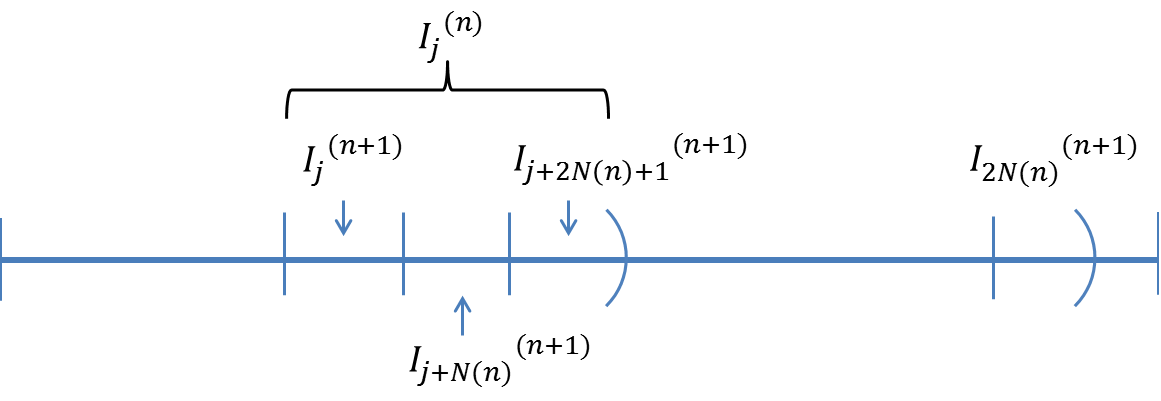
\includegraphics[scale=0.4]{1}
\end{figure}

The construction is basically "cutting the column into three, putting a spacer above the middle column, and stacking from left to right." We inductively construct the columns $C_0, C_1, C_2 \cdots$.
\s

Let \textbf{column}($C$) be a finite sequence of disjoint intervals of the same length. Each interval($I$) is called a \textbf{level} and the number of intervals in a column is called the \textbf{height}($h$) of the column.
\s

First, let $C_0$ denote the column consisting of a single interval $I_{0,0} = [0,\frac{2}{3})$. Then $h_0 =1$.
\s

Construction of $C_1$ : divide $C_0$ into three disjoint subintervals and put a spacer $S_0 = [2/3, 8/9)$. Then the union of all the intervals is $[0,8/9)$, and $h_1 =4$.
\s

We obtain $C_{n+1} = C_{n}$. $C_n$ has $(3^{n+1}-1)/2$ intervals, each of length $2\cdot 3^{-n-1}$, and the union of each levels is $[0,1-3^{-n-1}$. To obtain $C_{n+1}$, subdivide each interval equally into three and define spacer $S_n = [1-3^{-n-1},1- \frac{2}{3}3^{-n-1})$.
\s

Now define $T_{C_n}$ (for $n\geq 2$) be the map defined on $[0,1)$ by
\begin{align*}
T_{C_n}(x) = \begin{cases} \begin{array}{cl}
x & \text{if } x\in [1-1/3^{n+1},1) \\
x - \frac{1}{2} - \frac{5}{6} \frac{1}{3^n} & \text{if } x\in S_n \\
x + \frac{1}{2} & \text{if } x\in I^{(n)}_{2\cdot 3^{n-1}} \\
x- 1 + \frac{5}{3} \frac{1}{3^n} & \text{if } x\in I^{(n)}_{N(n)} \\
x + \cdots & \text{if otherwise}  
\end{array}
\end{cases}
\end{align*}
(has to complete this... but for form is too complicated!!) That is, $T_{C_n}$ is 'going up one level' where the levels are as displayed in the figure below.
\s

Define $T$, the Chac\'{o}n map as the limit of $T_{C_n}$.

\begin{figure}[h]
	\centering
	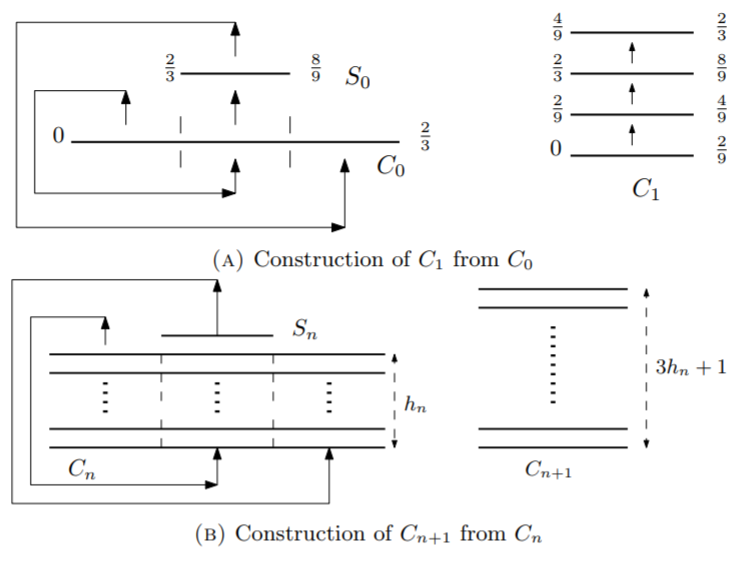
\includegraphics[scale=0.66]{2}
\end{figure}
\s

\digression


\newday

(1st November, Thursday)
\s

(Will be showing that $([0,1), \borel, \mu, T)$ is a measure preserving system in the example sheet 2.)
\s

\lem Consider $([0,1), \borel, \mu, T)$ where $m$ is the Lebesgue measure and $T$ is Chac\'{o}n map. Then $\forall$ $n,j$, we have
\begin{align*}
& m(I^{(n)}_j \cap T^{N(n)} I^{(n)}_j) \geq \frac{1}{3}m(I_j^{n}) \\
& m(I^{(n)}_j \cap T^{N(n)+1} I^{(n)}_j) \geq \frac{1}{3}m(I_j^{n})
\end{align*}
\begin{proof}
\pf Note 
\begin{align*}
& I_j^{(n)} = I_{j}^{(n+1)} \cup I_{j+N(n)}^{(n+1)} \cup I_{j+2N(n)+1}^{n+1} \\
\text{and} \quad & T^{N(n)} I_j^{(n+1)}  = I^{(n+1)}_{j+N(n)} \\
\text{and} \quad & T^{N(n)+1} I^{(n+1)}_{j+N(n)} = I^{(n+1)}_{j+2N(n)+1}
\end{align*}
Thus $I^{(n)}_j \cap T^{N(n)} I_j^{(n)} \supset I^{(n+1)}_{j+N(n)}$ and $I^{(n)}_j \cap T^{N(n)+1} I^{(n)}_j \supset I^{(n+1)}_{j+2N(n)+1}$.

\eop
\end{proof}
\s

\thm $([0,1), \borel, \mu, T)$ is not mixing.
\begin{proof}
\pf Consider $A= I^{(2)}_1$ then $m(A) = 2/9$. For $n\geq 2$, $A$ is the union of some intervals of the form $I^{(n)}_j$. Apply the lemma to each of these.
\begin{align*}
m(A\cap T^{N(n)} A) \geq \frac{1}{3} m(A) = \frac{3}{2} m(A)^2
\end{align*}
this contradicts the definition of mixing.

\eop
\end{proof}
\s

\thm  $([0,1), \borel, \mu, T)$ is weak mixing.
\begin{proof}
\pf Let $f\in L^2$ such that $f\circ T = \lambda f$ a.e. We aim to show that $f$ is constant a.e., then this implies that the system is weak mixing, by a theorem presented earlier. Note that $|\lambda| =1$.

\quad Fix $\epsilon >0$ sufficiently small,
\begin{proof}
e.g. $\epsilon < 1/12$ and
\begin{align*}
m(x\in [0,1) : |f(x)| >2) > 10\epsilon
\end{align*}
This might require replacing $f$ by a suitable constant multiple. 
\end{proof}
By Lousin's theorem, there is $h :[0,1] \rightarrow \mathbb{C}$ continuous such that $m(x\in [0,1) : f(x) \neq h(x)) < \epsilon$. Then if $n$ is sufficiently large, then $|h(x_1)-h(x_2)| < \epsilon$ whenever $|x_1 - x_2| < \frac{2}{3^n}$, and in particular this holds  when $x_1,x_2 \in I_j^{(n)}$ for some $j$. The intervals $I^{(n)}_j$ fill at least half of $[0,1)$. Therefore by pigeon hole principle, $\exists$ $j$ s.t. $m(x\in I^{(n)}_j : f(x) \neq h(x)) < 2\epsilon m(I^{(n)}_j)$. Let $z = f(x')$ for some $x' \in I^{(n)}_j$ such that $f(x') = h(x')$. Then
\begin{align*}
m(x\in I^{(n)}_j : |f(x) - \lambda^{N(n)}z| < \epsilon) \geq m\big( y \in I^{(n)}_j : T^{N(n)} y \in I^{(n)}_j \text{ and } f(y) = h(y) \big) 
\end{align*}
\begin{subproof}
: denote $A = \{ y \in I^{(n)}_j : T^{N(n)} y \in I^{(n)}_j \text{ and } f(y) = h(y) \}$, $B = \{ x\in I^{(n)}_j : |f(x) - \lambda^{N(n)}z| < \epsilon\}$. If $y\in A$, then $x = T^{N(n)} y \in I^{(n)}_j$ and 
\begin{align*}
f(x) = f(T^{(n)} y) = \lambda^{N(n)} f(y) = \lambda^{N(n)} h(y)
\end{align*}
Since $|h(y)-z| < \epsilon$, $|f(x) - \lambda^{N(n)}z| < \epsilon$, so $x\in B$. 
\end{subproof}
Hence
\begin{align*}
m(A) & \geq m(I_j^{(n)} \cap T^{N(n)}I^{(n)}_j)  - m(y \in I^{(n)}_j : f(y) \neq h(y)) \\
& \geq \frac{1}{3} m(I^{(n)}_j) - 2\epsilon m(I^{(n)}_j)
\end{align*}
Since $\epsilon < 1/12$, has $\frac{1}{3} > 2\epsilon$, so $m(A) >0$, i.e. $\exists$ $x\in I^{(n)}_j$ such that
\begin{align*}
f(x)  = h(x) \quad \text{and} \quad |f(x) - \lambda^{N(n)} z| < \epsilon
\end{align*}
and therefore $|f(x)-z| < \epsilon$ (as $z = f(T^n( x')) = f(x')$ for some $x' \in I^{(n)}_j$), thus $|z-\lambda^{N(n)}z| < 2\epsilon$.

\quad We will show in a minute that $|z| \geq 1$. If this is true, then
\begin{align*}
|1-\lambda^{N(n)}| < 2\epsilon
\end{align*} 
and same argument using the second claim in the lemma gives
\begin{align*}
|1- \lambda^{N(n)+1}| < 2\epsilon
\end{align*}
Hence :
\begin{align*}
|\lambda^{N(n)} - \lambda^{N(n)+1}| < 4\epsilon \quad \Rightarrow \quad |1-\lambda| < 4\epsilon
\end{align*}
Taking $\epsilon \searrow 0$< we get $\lambda =1$.

We now have to show that $|z| \geq 1$.
\begin{subproof}
 Recall $m(x\in I^{(n)}_j : |f(x)-z| > \epsilon) < 2\epsilon m(I^{(n)}_j)$. Using $T^{i-j}I_j^{(n)} = I^{(n)}_i$ we get
\begin{align*}
m(x\in I^{(n)}_j : |f(x) - \lambda^{i-j} z| &\leq \epsilon) \geq m(x\in [0,1) : |f(x)| > |z|+ \epsilon) \\
&\leq \sum_{i=1}^{N(n)} 2\epsilon m(I^{(n)}_i) + m([0,1) \backslash \cup_i I_i^{(n)}) \leq 2\epsilon + \frac{2}{3^n}
\end{align*}
\end{subproof}
\end{proof}
\s

\newday

(3rd November, Saturday)
\s

\textbf{Recall :}

$([0,1),\borel,m,T)$ a Chac\'{o}n map, $I_j^{(n)}$ intervals, $j=1,\cdots, N(n)$. To show this is a weak mixing, we aimed to show $f\circ T = \lambda f$ a.e. implies $f$ is constant a.e.
\s

So far, we prove : $\forall \epsilon >0$, $\forall n$ sufficiently large, $\exists z = z_{n,\epsilon} \mathbb{C}$ and $\exists j \in \{1, \cdots, N(n)\}$ such that
\begin{align*}
m(x\in I_j^{(n)}: |f(x) -z| > \epsilon ) < 2\epsilon m(I_j^{(n)})
\end{align*}
We also proved $\lambda =1$, provided we can show $|z_{n,\epsilon} \geq 1|$ for any $\epsilon >0$ and sufficiently large $n$.

(Using $T^{j-i}I_j^{(n)} = I_i^{(n)}$ and $|f(T^{i-j}x)| = |f(x)|$)
\s

\quad Summing these up for $i=1,\cdots, N(n)$, we get
\begin{align*}
m(x\in [0,1) : |f(x)| \leq |z| +\epsilon) \geq (1-2\epsilon) \sum_{i=1}^{N(n)} m(I^{(n)}_j) = (1-2\epsilon) (1-3^{-n})
\end{align*}
If $n$ is sufficiently large, then
\begin{align*}
m(x\in[0,1) : |f(x)| \leq 1+ \epsilon) \geq 1-10\epsilon
\end{align*}
Comparing this with our ssumption on $\epsilon$ at the beginning of the proof, we get $|z| \geq 1$, so now we get $|z| =1$. Thus $f(T^{i-j}x) = f(x)$.

\quad The same argument using this instead of $|f(T^{i-j}x)| = |f(x)|$ gives
\begin{align*}
m(x\in [0,1) : |f(x) - z_{n,\epsilon} | \leq \epsilon ) \geq (1-2\epsilon) (1-3^{-n}) \quad \cdots\cdots (\dagger)
\end{align*}
Choose sequence $\epsilon_m\rightarrow 0$ and $n_m\\rightarrow \infty$ such that $z_{n_m, \epsilon_m}$ converges to a complex number $\tilde{z}$(in fact, we have to first check that $z_{n,\epsilon}$ has a bounded subsequence), by Bozanno-Weierstrasss. If $m$ is sufficiently large (depending on $\delta >0$) then
\begin{align*}
m(x\in [0,1) : |f(x)-\tilde{z}| < \delta ) > 1-\delta
\end{align*}
if we use $(\dagger)$ for $n_m$ and $\epsilon_m$.

\section*{9. Entropy}

\textbf{Bernoulli Shift : } Let $(P_1, P_2,\cdots, P_d)$ be a probability vector. The \textbf{$(P_1, \cdots, P_d)$-Bernoulli shift} is the MPS
\begin{align*}
\big( \{1,\cdots, d\}^{\mathbb{Z}}, \borel, \mu_{P_1,\cdots, P_d},\sigma \big)
\end{align*}
where $\mu_{P_1,\cdots, P_d}$ is the product measure with $(P_1,\cdots, P_d)$ on the coordinates and $\sigma$ is the shift map.
\s

\defi The MPS $(X_1, \borel_1, \mu_1, T_1)$ and $(X_2,\borel_2, \mu_2, T_2)$ are called \textbf{isomorphic}, if there are maps
\begin{align*}
S_1 : X_1\rightarrow X_2,\quad S_2 : X_2 \rightarrow X_1
\end{align*}
such that $S_1 \circ S_2 = id_{X_2}$ a.e., $S_2 \circ S_1 = id_{X_1}$ a.e., $(S_1)_* \mu_1 =\mu_2$, $(S_2)_* \mu_2 =\mu_1$ and $T_1 \circ S_2 = T_1 \circ T_2$ a.e.
\s

\textbf{The Question :} Are the $(\frac{1}{2}, \frac{1}{2})$ and $(\frac{1}{3},\frac{1}{3},\frac{1}{3})$ Bernoulli-shift isomorphic?
\s

This question does not seem very difficult, but this had been unsolved for a long time. These two shifts have "the same" Koopman operators, and moreover Meshalkin proved that $(\frac{1}{4},\frac{1}{4},\frac{1}{4},\frac{1}{4})$ and $(\frac{1}{2},\frac{1}{8},\frac{1}{8},\frac{1}{8},\frac{1}{8})$-Bernoulli shifts are isomorphic. This problem was finally solved by Kolmogorov. He proved that these two systems are not isomorphic by attaching a quantity called \emph{entropy}, which should be preserved by isomorphism, on each system and by showing they are not equal. Later, Ornstein showed that two Bernoulli shifts are isomorphic if and only if they have the same entropy. Actually, the introduction of notion of entropy in measure preserving systems was the starting point of ergodic theory being identified as an independent subject, so the importance of entropy in the field of ergodic theory cannot be overemphasize.
\s

Let us do some actual mathematics now. We define the entropy as the measure of the amount how difficult it is to predict the system.
\s

\defi Let $(X,\borel, \mu)$ be a probability space. A \textbf{countable measurable partition} is a collection of measurable sets $A_1, A_2, \cdots$ such that $A_i \cap A_j =\phi$ for all $i\neq j$ and $\bigcup A_i = X$. The sets $A_i$ are called the atoms of partition. 

\quad The \textbf{join} or \textbf{coarsest common refinement} of two countable measurable partiotion $\xi, \eta$ is
\begin{align*}
\xi \vee \eta = \{A \cap B : A\in \xi, B \in \eta \}
\end{align*}

\quad Define a function
\begin{align*}
H(p_1, \cdots, p_d) = - \sum_{j=1}^d p_j \log (p_j)
\end{align*}
for all probability vector $(p_1, \cdots, p_d)$ with the convention $0 \cdot \log 0 =0$. The \textbf{entropy} of a countable measurable partition $\xi$ is
\begin{align*}
H_{\mu}(\xi) = H(\mu(A_1), \mu(A_2), \cdots)
\end{align*}
where $\xi = \{A_1, A_2, \cdots \}$.

\quad The \textbf{conditional entropy} of $\xi = \{A_1, A_2, \cdots \}$ relative to $\eta = \{B_1, B_2, \cdots \}$ is 
\begin{align*}
H_{\mu} (\xi | \eta) = \sum_{n=1}^{\infty} \mu(B_n) \cdot H\Big( \frac{\mu(A_1 \cap B_n)}{\mu(B_n)},\frac{\mu(A_2 \cap B_n)}{\mu(B_n)},\cdots \Big)
\end{align*}
This is the average average of entropy conditioned on each partition of 
\s

$\star$ Very Useful Interpretations : 

\quad Entropy of $\xi$ provides the amount of information we can obtain from an experiment $\xi$. Conditional entropy of $\xi$ relative to $\eta$ provides the amount of information we can get from $\xi$ given the information about experiment $\eta$. Entropy of join $\xi \vee \eta$ gives the amount of information we can get if we perform both experiments $\xi$ and $\eta$.
\s

\lem
\begin{itemize}
\item[(1)] $H_{\mu} (\xi) \geq 0$.
\item[(2)] The value of $H_{\mu}(\xi)$ is maximal among partition $\xi$ with $k$ atoms if all atoms have the same measure $\frac{1}{k}$.
\item[(3)] $H_{\mu}(\{A_1, \cdots, A_k \}) = H_{\mu}(A_{\rho (1)}, \cdots, A_{\rho (k)})$ for all permutations $\rho \in \text{Sym}(\{1,\cdots,k\})$.
\item[(4)] $H_{\mu} (\xi \vee \eta) = H_{\mu}(\xi) + H_{\mu}(\eta |\xi)$. This is called \emph{chain rule.}
\end{itemize}
\begin{proof}
\pf \begin{itemize}
\item (1) is trivial and (2) is going to be proved shortly using Jensen's inequality.
\item (3) and (4) are going to be proved later, in more general setting.
\end{itemize}
\end{proof}
\s

\textbf{Khinchin)} Let $H_{\cdot}(\cdot) : P(X) \times \borel$ be a function satisfying the conditions (1)-(4) of the lemma, where $P(X)$ is the set of Borel probability measures on $(X,\borel)$. Then $H_{\cdot}(\cdot)$ is uniquely determined by these properties, up to a multiplication of a scalar factor.
\s

\newday
\s

(6th November, Tuesday)

\defi A function $[a,b] \rightarrow \reals \cup \{ \infty \}$ is \textbf{convex}, if $\forall x \in (a,b)$, $\exists \alpha_x \in \reals$ such that
\begin{align*}
f(y) \geq f(x) + \alpha_x (y-x) \quad \forall y \in [a,b]
\end{align*}
$f$ is \textbf{strictly convex} if the equality occurs only for $x=y$. 
\s

\textbf{Remark :} If $f$ is $C^2([a,b])$ and $f''(x) >0$ for all $x\in (a,b)$, then $f$ is strictly convex.
\s

\textbf{Jensen's inequality)} Let $f:[a,b] \rightarrow \reals \cup \{\infty\}$ be a convex function. Let $p_1, p_2, \cdots$ be a probability vector (possibly countably infinite). Let $x_1, x_2, \cdots \in [a,b]$. Then
\begin{align*}
f(p_1 x_1 + p_2 x_2 + \cdots) \leq \sum_i p_i f(x_i)
\end{align*}
If $f$ is strictly convex, then equality occurs \emph{iff} those $x_i$ for which $p_i >0$ coincide.
\s

\textbf{Claim :} Let $(X,\borel, \mu)$ be a probability space. Let $\xi$ be a measurable partition with $k$ atoms. Then
\begin{align*}
H_{\mu}(\xi) \leq \log (k)
\end{align*}
and equality occurs only if each atom of $\xi$ has measures $\frac{1}{k}$.
\begin{proof}
\pf Apply Jensen's inequality to the function $x\mapsto x \log (x)$ with weights $p_i = \frac{1}{k}$ at the point $\mu(A_i)$, where $A_i$ are the atoms of $\xi$. Note,
\begin{align*}
& \sum p_i \mu(A_i) = \frac{1}{k} \sum \mu(A_i) = \frac{1}{k} \\
\Rightarrow \quad & \frac{1}{k} \log (\frac{1}{k}) \leq \sum \frac{1}{k} \mu(A_i) \log (\mu(A_i))
\end{align*}
so
\begin{align*}
\log k \geq \sum (-1) \mu(A_i) \log \mu(A_i) = H_{\mu}(\xi)
\end{align*}

\eop
\end{proof}

\s

\defi Let $(X, \borel, \mu)$ be a probability space and let $\xi$ be a countable measurable partition. The \textbf{information function} of $\xi$ is
\begin{align*}
I_{\mu} (\xi) : & X \rightarrow \reals \cup \{\infty \} \\
& x\mapsto -\log \mu \big( [x]_{\xi} \big)
\end{align*}
where $[x]_{\xi}$ is the atom of $\xi$ where $x$ belongs.

\quad If $\eta$ is another partition, then the \textbf{conditional information function} of $\xi$ relative to $x$ is
\begin{align*}
I_{\mu} (\xi | \eta) (x)  = - \log \frac{\mu \big( [x]_{\xi \vee \eta} \big)}{\mu \big( [x]_{\eta} \big)}
\end{align*}
\s

It is apparent that the information function is related to entropy. This is summarized in the following lemma.
\s

\lem With notation as above,
\begin{align*}
& H_{\mu}(\xi) = \int I_{\mu} (\xi) d \mu \\
& H_{\mu}(\xi | \eta) = \int I_{\mu} (\xi | \eta) d \mu
\end{align*}
\begin{proof}
\pf The first equality is direct from the definition. For the second equality,
\begin{align*}
I_{\mu} (\xi |\eta) d\mu &= \sum_{A\in \xi, B \in \eta} \int_{A \cap B} I_{\mu}(\xi | \eta) d\mu = - \sum_{A \in \xi, B\in \eta} \mu(A\cap B) \log \Big( \frac{\mu(A \cap B)}{\mu(B)}\Big) \\
&= -\sum_{B\in \eta} \mu(B) \cdot \sum_{A\in \xi} \frac{\mu(A\cap B)}{\mu(B)} \log \Big( \frac{\mu(A\cap B)}{\mu(B)} \Big)
\end{align*}

\eop
\end{proof}
\s

One reason we use information function is that it is much easier to prove chain rule with information function.
\s

\lem \emph{(Chain rule)} Let $(X,\borel, \mu)$ be a probability space and let $\xi, \eta, \lambda$ be countable measurable partitions. Then
\begin{align*}
I_{\mu} (\xi \vee \eta | \lambda)(x) &= I_{\mu}(\xi | \lambda) (x) + I_{\mu}(\eta | \xi \vee \lambda)(x) \quad \forall x \in X \\
H_{\mu} (\xi \vee \eta | \lambda) &= H_{\mu}(\xi | \lambda)  + H_{\mu}(\eta | \xi \vee \lambda)
\end{align*}
\begin{proof}
\pf For the first equality,
\begin{align*}
I_{\mu} (\xi \vee \eta |\lambda) (x)  &= \log \frac{\mu ([x]_{\lambda})}{\mu([x]_{\xi \vee \eta \vee \lambda})} \\
I_{\mu} (\xi |\lambda) (x)  &= \log \frac{\mu ([x]_{\lambda})}{\mu([x]_{\xi \vee \lambda})} \\
I_{\mu} (\eta |\lambda \vee \xi) (x)  &= \log \frac{\mu ([x]_{\xi \vee \lambda})}{\mu([x]_{\xi \vee \eta \vee \lambda})} \\
\end{align*}
and this proves the chain rule for information function.

\quad The second equality follows from the first equality by integration the information function (as in the previous lemma).

\eop
\end{proof}
\s

The following inequality is very important in theory of mathematics of information.
\s

\lem Let notation be as above. Then
\begin{align*}
H_{\mu}(\xi | \eta) \geq H_{\mu}(\xi | \eta \vee \lambda)
\end{align*}

"The amount of information obtained from $\xi$ given $\eta$ is larger than information obtained from $\xi$ given $\eta$ and $\lambda$."
\begin{proof}
\pf 
\begin{align*}
H_{\mu}(\xi | \eta \vee \lambda) &= \sum_{A \in \xi, B \in \eta, C \in \lambda} \mu(A\cap B \cap C) \log \Big( \frac{\mu(B\cap C)}{\mu(A\cap B \cap C)}\Big) \\
H_{\mu}(\xi | \eta ) &= \sum_{A \in \xi, B \in \eta} \mu(A\cap B ) \log \Big( \frac{\mu(B)}{\mu(A\cap B )}\Big)
\end{align*}
It is enough to show that for all fixed $A \in \xi$, $B\in \eta$, we have
\begin{align*}
\mu(A\cap B) \log \Big( \frac{\mu(B)}{\mu(A\cap B)}\Big) \geq \sum_{C \in \lambda} \mu(A \cap B \cap C) \log \Big( \frac{\mu(B\cap C)}{\mu(A\cap B \cap C)} \Big)
\end{align*}
To see this, apply Jensen's inequality for $x\mapsto x\log x$ at points $\frac{\mu(A\cap B\cap C)}{\mu(B \cap C)}$ for $C \in \lambda$ with weights $\frac{\mu(B\cap C)}{\mu(B)}$. Write
\begin{align*}
\sum_{C\in \lambda } \frac{\mu(B\cap C)}{\mu(B)} \cdot \frac{\mu(A\cap B \cap C)}{\mu(B\cap C)} = \frac{1}{\mu(B)} \sum_{C\in \lambda} \mu(A\cap B \cap C) = \frac{\mu(A\cap B)}{\mu(B)}
\end{align*}
and application of Jensen gives
\begin{align*}
\frac{\mu(A\cap B)}{\mu(B)}\cdot \log \Big( \frac{\mu(A\cap B)}{\mu(B)} \Big) \leq \sum_{C\in \lambda} \frac{\mu(B\cap C)}{\mu(B)} \cdot \log\Big( \frac{\mu(A\cap B \cap C)}{\mu(B\cap C)} \Big)
\end{align*}
and therefore
\begin{align*}
\mu(A\cap B)\cdot \log \Big( \frac{\mu(A\cap B)}{\mu(B)} \Big) \leq \sum_{C\in \lambda} \mu(B\cap C) \cdot \log \Big( \frac{\mu(A\cap B \cap C)}{\mu(B\cap C)} \Big)
\end{align*}

\eop
\end{proof}
\s

\cor $H_{\mu}(\xi) \leq H_{\mu}(\xi \vee \eta) \leq H_{\mu}(\xi) + H_{\mu}(\eta)$.
\begin{proof}
\pf Using the chain rule, obtain
\begin{align*}
H_{\mu}(\xi \vee \eta) = H_{\mu} (\xi)  + H_{\mu}(\eta | \xi)
\end{align*}
and form the previous lemma, has $H_{\mu}(\eta |\xi) \leq H_{\mu}(\eta)$

\eop
\end{proof}
\s

\newday

(8th November, Thursday)
\s

\lem Let $(X,\borel, \mu, T)$ be an MPS. Let $\xi, \eta$ be countable measurable partitions. Then :
\begin{align*}
& I_{\mu}(T^{-1}\xi | T^{-1} \eta ) = I_{\mu}(\xi | \eta)(Tx) \\
& H_{\mu}(T^{-1} \xi | T^{-1} \eta) = H_{\mu}(\xi | \eta)
\end{align*}
where $T^{-1} \xi$ is the partition whose atoms are $T^{-1}([x]_{\xi})$.

\begin{proof}
\pf Has 
\begin{align*}
I_{\mu}(T^{-1} \xi | T^{-1} \eta)(x)  = -\log \Big( \frac{\mu([x]_{T^{-1}\xi \vee T^{-1}\eta} )}{\mu([x])_{T^{-1}\eta}} \Big)
\end{align*}
Note
\begin{align*}
T^{-1} \xi \vee T^{-1}\eta = T^{-1}(\xi \vee \eta) \quad \text{and} \quad [x]_{T^{-1} \xi \vee T^{-1}\eta} = T^{-1} [Tx]_{\xi \vee \eta}
\end{align*}
hence $\mu([x]_{T^{-1} \xi \vee T^{-1}\eta}) = \mu([Tx]_{\xi \vee \eta})$ by the measure preserving property. Similarly $\mu([x]_{T^{-1}\eta}) = \mu ([Tx]_{\eta})$. Then $I_{\mu}(T^{-1}\xi | T^{-1} \eta ) = -\log \Big( \frac{\mu([x]_{T^{-1}\xi \vee T^{-1}\eta} )}{\mu([x])_{T^{-1}\eta}} \Big) =  I_{\mu}(\xi | \eta)(Tx)$

\quad The statement on $H_{\mu}$ follows by integrating $I_{\mu}$

\eop
\end{proof}
\s

\cor Writing $\xi_m^n = T^{-m} \xi \vee T^{-(m+1)}\xi \vee \cdots \vee T^{-n} \xi$, has
\begin{align*}
H_{\mu}(\xi_0^{n+m-1}) \leq H_{\mu}(\xi_0^{n-1}) + H_{\mu}(\xi_0^{m-1})
\end{align*}
\begin{proof}
\pf Note that $\xi_0^{n+m-1} = \xi_0^{n-1} \vee \xi_n^{n+m-1}$. So we have
\begin{align*}
H_{\mu}(\xi_0^{n+m-1}) &\leq H_{\mu}(\xi_0^{n-1})+ H_{\mu}(\xi_n^{n+m-1}) = H_{\mu}(\xi_0^{n-1}) + H_{\mu}(T^{-n}\xi_0^{m-1}) \\
&= H_{\mu}(\xi_0^{n-1}) + H_{\mu}(\xi_0^{m-1})
\end{align*}
where the last equality follows from the previous lemma.

\eop
\end{proof}
\s

\lem \emph{(Felate's lemma)} Let $(a_n)\subset \reals$ be a subadditive sequence, that is
\begin{align*}
a_{n+m} \leq a_n + a_m \quad \forall n,m
\end{align*}
Then $\lim_{n\rightarrow \infty} a_n/n$ exists and equals $\inf_{n} a_n /n $.
\begin{proof}
\textbf{proof sketch)} Need to show that $\limsup_{n\rightarrow \infty} \frac{a_n}{n} \leq \frac{a_{n_0}}{n_0}$ for all $n_0$. For each fixed $n_0$, we can write $n = j(n)n_0 + i(n)$, where $i(n) \in [0,n_0-1]$. Iterate sub-additivity to get $a_n \leq j(n) a_{n_0} + a_{i(n)}$.

\quad See the online note for the full proof.
\end{proof}
\s

\defi Let $(X,\borel, \mu, T)$ be an MPS. Let $\xi, \eta$ be countable measurable partitions such that $H_{\mu}(\xi) < \infty$. The \textbf{entropy of the MPS w.r.t. $\xi$} is :
\begin{align*}
h_{\mu} (\xi) = \lim_{n\rightarrow \infty} \frac{H_{\mu}(\xi_0^{n-1})}{n} = \inf_n \frac{H_{\mu}(\xi_0^{n-1})}{n}
\end{align*}
whose existence of the limit is guaranteed by \emph{Felate's lemma}.(in fact, $\frac{H_{\mu}(\xi_0^{n-1})}{n}$ is a monotone decreasing sequence - will show in the example sheet)

\quad The \textbf{entropy of the MPS} is $h_{\mu}(T) = \sup_{\xi : H_{\mu}(\xi)<\infty} h_{\mu}(T|\xi)$.
\s

$h_{\mu} (\xi)$ expresses how fast we can learn information from a particular experiment $\xi$, and $h_{\mu}(T)$ is the maximal information we can obtain from the system when an appropriate experiment is chosen.
\s

The problem of this definition is that it is generally difficult to find out the supremum $\sup_{\xi : H_{\mu}(\xi)<\infty} h_{\mu}(T|\xi)$ - since this requires computing entropy w.r.t $\xi$ for each $\xi$. The good news is that (at least for the Bernoulli shifts), if we can find a partition that satisfies a particular property(so called \textbf{2-sided generator}), then in fact the supremum is achieved by the partition.
\s

\defi Let $(X,\borel, \mu, T)$ be an invertible MPS. Let $\xi \subset \borel$ be a countable measurable partitions. We say that $\xi$ is a \textbf{2-sided generator} if $\forall A\in \borel$ and $\forall \epsilon >0$, $\exists k\in \mathbb{Z}_{>0}$ such that $\exists A'\in \sigma( \xi^k_{-k} )$ and $\mu(A \triangle A') <\epsilon$.
\s

\thm \emph{(Kolmogorov-Sinai)} Let $(X,\borel, \mu, T)$ be an \emph{invertible} measure preserving system. Let $\xi$ be a countable measurable partition with $H_{\mu}(\xi) < \infty$, which is a 2-sided generator. Then
\begin{align*}
h_{\mu}(T) = h_{\mu}(T,\xi)
\end{align*}
\s

We delay the proof of this theorem until next lecture. Instead, we start to compute something useful.
\s

\textbf{Example :} Let $(\{1,2,\cdots, k\}^{\mathbb{Z}}, \borel, \mu, \sigma)$ be the $(p_1, \cdots, p_k)$-Bernoulli shift. Let $X =\{1,2,\cdots, k\}^{\mathbb{Z}}$.
\begin{itemize}
\item \textbf{Claim :} The partition $\xi = \{ \{x\in X: x_0 =j \} : j=1, \cdots, k \}$ is a 2-sided generator.
\begin{subproof}
\pf The collection of sets
\begin{align*}
\{ A\in \borel : \forall \epsilon, \,\, \exists k \,\, \exists A' \in \xi^{k}_{-k} \text{ with } \mu(A\triangle A') < \epsilon \} \subset \sigma(\xi) \subset \borel
\end{align*}
is a $\sigma$-algebra, and it contains cylinder sets. Hence it is equal to $\borel$, as $\borel$ is generated by cylinder sets.

\eop
\end{subproof}
\s

\item \textbf{Claim :} With $\xi$ defined as above, we have 
\begin{align*}
H_{\mu}(\xi | \xi_{1}^n) = H(p_1, p_2, \cdots, p_k) = -p_1 \log p_1 -\cdots -p_k \log p_k
\end{align*}
for all $n \in \mathbb{Z}_{\geq 0}$.
\begin{subproof}
\pf Calculate the information function : 
\begin{align*}
I_{\mu}(\xi | \xi_1^n) (x)  = \log \Big( \frac{\mu([x]_{\xi_1^n})}{\mu([x]_{\xi_0^n})} \Big)
\end{align*}
Note $[x]_{\xi_0^n} = \{y\in X : y_0=x_0, \cdots, y_n =x_n \}$, so $\mu([x]_{\xi_0^n}) = p_{x_0}\cdots p_{x_n}$. Similarly, has $\mu([x]_{\xi_1^n})=p_{x_1} \cdots p_{x_n}$, and
\begin{align*}
I_{\mu}(\xi|\xi_1^n) (x) = - \log p_{x_0} 
\end{align*}
therefore $H_{\mu} (\xi |\xi_1^n) = \sum_{j=1}^{k} p_j (-\log (p_j)) = H(p_1, \cdots, p_k)$. 

\eop
\end{subproof}
\s

\item Hence
\begin{align*}
H_{\mu}(\xi_1^{n-1}) &= H_{\mu}(\xi_{n-1}^{n-1}) + H_{\mu}(\xi_{n-2}^{n-2} | \xi_{n-1}^{n-1}) + H_{\mu}(\xi_{n-3}^{n-3} | \xi_{n-2}^{n-1}) + \cdots + H_{\mu}(\xi | \xi^{n-1}_{1}) \quad (\text{Chain rule}) \\
&= H_{\mu}(\xi) + H(\xi |\xi_1^1) + \cdots + H_{\mu}(\xi | \xi_1^{n-1}) \quad (\text{invariance, first lemma of the day}) \\
&= nH(p_1, \cdots, p_k)
\end{align*}
Divide by $n$ and take the limit, 
\begin{align*}
h_{\mu}(T) = h_{\mu}(T,\xi) = H(p_1, \cdots, p_k)
\end{align*}

So the entropy of $(1/2,1/2)$ shift is $\log2$ and $(1/3,1/3,1/3)$ shift is $\log3$ - which shows that two systems cannot be isomorphic.
\end{itemize}
















\end{document}
